% Options for packages loaded elsewhere
\PassOptionsToPackage{unicode}{hyperref}
\PassOptionsToPackage{hyphens}{url}
\PassOptionsToPackage{dvipsnames,svgnames,x11names}{xcolor}
%
\documentclass[
  letterpaper,
  DIV=11,
  numbers=noendperiod]{scrartcl}

\usepackage{amsmath,amssymb}
\usepackage{iftex}
\ifPDFTeX
  \usepackage[T1]{fontenc}
  \usepackage[utf8]{inputenc}
  \usepackage{textcomp} % provide euro and other symbols
\else % if luatex or xetex
  \usepackage{unicode-math}
  \defaultfontfeatures{Scale=MatchLowercase}
  \defaultfontfeatures[\rmfamily]{Ligatures=TeX,Scale=1}
\fi
\usepackage{lmodern}
\ifPDFTeX\else  
    % xetex/luatex font selection
\fi
% Use upquote if available, for straight quotes in verbatim environments
\IfFileExists{upquote.sty}{\usepackage{upquote}}{}
\IfFileExists{microtype.sty}{% use microtype if available
  \usepackage[]{microtype}
  \UseMicrotypeSet[protrusion]{basicmath} % disable protrusion for tt fonts
}{}
\makeatletter
\@ifundefined{KOMAClassName}{% if non-KOMA class
  \IfFileExists{parskip.sty}{%
    \usepackage{parskip}
  }{% else
    \setlength{\parindent}{0pt}
    \setlength{\parskip}{6pt plus 2pt minus 1pt}}
}{% if KOMA class
  \KOMAoptions{parskip=half}}
\makeatother
\usepackage{xcolor}
\setlength{\emergencystretch}{3em} % prevent overfull lines
\setcounter{secnumdepth}{-\maxdimen} % remove section numbering
% Make \paragraph and \subparagraph free-standing
\ifx\paragraph\undefined\else
  \let\oldparagraph\paragraph
  \renewcommand{\paragraph}[1]{\oldparagraph{#1}\mbox{}}
\fi
\ifx\subparagraph\undefined\else
  \let\oldsubparagraph\subparagraph
  \renewcommand{\subparagraph}[1]{\oldsubparagraph{#1}\mbox{}}
\fi

\usepackage{color}
\usepackage{fancyvrb}
\newcommand{\VerbBar}{|}
\newcommand{\VERB}{\Verb[commandchars=\\\{\}]}
\DefineVerbatimEnvironment{Highlighting}{Verbatim}{commandchars=\\\{\}}
% Add ',fontsize=\small' for more characters per line
\usepackage{framed}
\definecolor{shadecolor}{RGB}{241,243,245}
\newenvironment{Shaded}{\begin{snugshade}}{\end{snugshade}}
\newcommand{\AlertTok}[1]{\textcolor[rgb]{0.68,0.00,0.00}{#1}}
\newcommand{\AnnotationTok}[1]{\textcolor[rgb]{0.37,0.37,0.37}{#1}}
\newcommand{\AttributeTok}[1]{\textcolor[rgb]{0.40,0.45,0.13}{#1}}
\newcommand{\BaseNTok}[1]{\textcolor[rgb]{0.68,0.00,0.00}{#1}}
\newcommand{\BuiltInTok}[1]{\textcolor[rgb]{0.00,0.23,0.31}{#1}}
\newcommand{\CharTok}[1]{\textcolor[rgb]{0.13,0.47,0.30}{#1}}
\newcommand{\CommentTok}[1]{\textcolor[rgb]{0.37,0.37,0.37}{#1}}
\newcommand{\CommentVarTok}[1]{\textcolor[rgb]{0.37,0.37,0.37}{\textit{#1}}}
\newcommand{\ConstantTok}[1]{\textcolor[rgb]{0.56,0.35,0.01}{#1}}
\newcommand{\ControlFlowTok}[1]{\textcolor[rgb]{0.00,0.23,0.31}{#1}}
\newcommand{\DataTypeTok}[1]{\textcolor[rgb]{0.68,0.00,0.00}{#1}}
\newcommand{\DecValTok}[1]{\textcolor[rgb]{0.68,0.00,0.00}{#1}}
\newcommand{\DocumentationTok}[1]{\textcolor[rgb]{0.37,0.37,0.37}{\textit{#1}}}
\newcommand{\ErrorTok}[1]{\textcolor[rgb]{0.68,0.00,0.00}{#1}}
\newcommand{\ExtensionTok}[1]{\textcolor[rgb]{0.00,0.23,0.31}{#1}}
\newcommand{\FloatTok}[1]{\textcolor[rgb]{0.68,0.00,0.00}{#1}}
\newcommand{\FunctionTok}[1]{\textcolor[rgb]{0.28,0.35,0.67}{#1}}
\newcommand{\ImportTok}[1]{\textcolor[rgb]{0.00,0.46,0.62}{#1}}
\newcommand{\InformationTok}[1]{\textcolor[rgb]{0.37,0.37,0.37}{#1}}
\newcommand{\KeywordTok}[1]{\textcolor[rgb]{0.00,0.23,0.31}{#1}}
\newcommand{\NormalTok}[1]{\textcolor[rgb]{0.00,0.23,0.31}{#1}}
\newcommand{\OperatorTok}[1]{\textcolor[rgb]{0.37,0.37,0.37}{#1}}
\newcommand{\OtherTok}[1]{\textcolor[rgb]{0.00,0.23,0.31}{#1}}
\newcommand{\PreprocessorTok}[1]{\textcolor[rgb]{0.68,0.00,0.00}{#1}}
\newcommand{\RegionMarkerTok}[1]{\textcolor[rgb]{0.00,0.23,0.31}{#1}}
\newcommand{\SpecialCharTok}[1]{\textcolor[rgb]{0.37,0.37,0.37}{#1}}
\newcommand{\SpecialStringTok}[1]{\textcolor[rgb]{0.13,0.47,0.30}{#1}}
\newcommand{\StringTok}[1]{\textcolor[rgb]{0.13,0.47,0.30}{#1}}
\newcommand{\VariableTok}[1]{\textcolor[rgb]{0.07,0.07,0.07}{#1}}
\newcommand{\VerbatimStringTok}[1]{\textcolor[rgb]{0.13,0.47,0.30}{#1}}
\newcommand{\WarningTok}[1]{\textcolor[rgb]{0.37,0.37,0.37}{\textit{#1}}}

\providecommand{\tightlist}{%
  \setlength{\itemsep}{0pt}\setlength{\parskip}{0pt}}\usepackage{longtable,booktabs,array}
\usepackage{calc} % for calculating minipage widths
% Correct order of tables after \paragraph or \subparagraph
\usepackage{etoolbox}
\makeatletter
\patchcmd\longtable{\par}{\if@noskipsec\mbox{}\fi\par}{}{}
\makeatother
% Allow footnotes in longtable head/foot
\IfFileExists{footnotehyper.sty}{\usepackage{footnotehyper}}{\usepackage{footnote}}
\makesavenoteenv{longtable}
\usepackage{graphicx}
\makeatletter
\def\maxwidth{\ifdim\Gin@nat@width>\linewidth\linewidth\else\Gin@nat@width\fi}
\def\maxheight{\ifdim\Gin@nat@height>\textheight\textheight\else\Gin@nat@height\fi}
\makeatother
% Scale images if necessary, so that they will not overflow the page
% margins by default, and it is still possible to overwrite the defaults
% using explicit options in \includegraphics[width, height, ...]{}
\setkeys{Gin}{width=\maxwidth,height=\maxheight,keepaspectratio}
% Set default figure placement to htbp
\makeatletter
\def\fps@figure{htbp}
\makeatother

\KOMAoption{captions}{tableheading}
\makeatletter
\makeatother
\makeatletter
\makeatother
\makeatletter
\@ifpackageloaded{caption}{}{\usepackage{caption}}
\AtBeginDocument{%
\ifdefined\contentsname
  \renewcommand*\contentsname{Table of contents}
\else
  \newcommand\contentsname{Table of contents}
\fi
\ifdefined\listfigurename
  \renewcommand*\listfigurename{List of Figures}
\else
  \newcommand\listfigurename{List of Figures}
\fi
\ifdefined\listtablename
  \renewcommand*\listtablename{List of Tables}
\else
  \newcommand\listtablename{List of Tables}
\fi
\ifdefined\figurename
  \renewcommand*\figurename{Figure}
\else
  \newcommand\figurename{Figure}
\fi
\ifdefined\tablename
  \renewcommand*\tablename{Table}
\else
  \newcommand\tablename{Table}
\fi
}
\@ifpackageloaded{float}{}{\usepackage{float}}
\floatstyle{ruled}
\@ifundefined{c@chapter}{\newfloat{codelisting}{h}{lop}}{\newfloat{codelisting}{h}{lop}[chapter]}
\floatname{codelisting}{Listing}
\newcommand*\listoflistings{\listof{codelisting}{List of Listings}}
\makeatother
\makeatletter
\@ifpackageloaded{caption}{}{\usepackage{caption}}
\@ifpackageloaded{subcaption}{}{\usepackage{subcaption}}
\makeatother
\makeatletter
\@ifpackageloaded{tcolorbox}{}{\usepackage[skins,breakable]{tcolorbox}}
\makeatother
\makeatletter
\@ifundefined{shadecolor}{\definecolor{shadecolor}{rgb}{.97, .97, .97}}
\makeatother
\makeatletter
\makeatother
\makeatletter
\makeatother
\ifLuaTeX
  \usepackage{selnolig}  % disable illegal ligatures
\fi
\IfFileExists{bookmark.sty}{\usepackage{bookmark}}{\usepackage{hyperref}}
\IfFileExists{xurl.sty}{\usepackage{xurl}}{} % add URL line breaks if available
\urlstyle{same} % disable monospaced font for URLs
\hypersetup{
  pdftitle={Problem Set 2},
  pdfauthor={Valerio Palagi, Lucia Pezzetti, Federico Testa},
  colorlinks=true,
  linkcolor={blue},
  filecolor={Maroon},
  citecolor={Blue},
  urlcolor={Blue},
  pdfcreator={LaTeX via pandoc}}

\title{Problem Set 2}
\author{Valerio Palagi, Lucia Pezzetti, Federico Testa}
\date{}

\begin{document}
\maketitle
\ifdefined\Shaded\renewenvironment{Shaded}{\begin{tcolorbox}[boxrule=0pt, breakable, enhanced, frame hidden, borderline west={3pt}{0pt}{shadecolor}, interior hidden, sharp corners]}{\end{tcolorbox}}\fi

\hypertarget{exercise-1}{%
\subsection{Exercise 1}\label{exercise-1}}

We consider the dataset \texttt{psych} which contains 24 cognitive tests
administered to 301 students (with ages ranging from 11 to 16) in a
suburb of Chicago: a group of 156 students (74 boys, 82 girls) from the
Pasteur School and a group of 145 students (72 boys, 73 girls) from the
Grant-White School.

\begin{verbatim}
  Case Sex  Age V1 V2 V3 V4 V5 V6 V7 V8 V9 V10 V11 V12 V13 V14 V15 V16 V17 V18
1    1   M 13.1 20 31 12  3 40  7 23 22  9  78  74 115 229 170  86  96   6   9
2    2   F 13.6 32 21 12 17 34  5 12 22  9  87  84 125 285 184  85 100  12  12
3    3   F 13.1 27 21 12 15 20  3  7 12  3  75  49  78 159 170  85  95   1   5
4    4   M 13.2 32 31 16 24 42  8 18 21 17  69  65 106 175 181  80  91   5   3
5    5   F 12.2 29 19 12  7 37  8 16 25 18  85  63 126 213 187  99 104  15  14
6    6   F 14.1 32 20 11 18 31  3 12 25  6 100  92 133 270 164  84 104   6   6
  V19 V20 V21 V22 V23 V24   group
1  16   3  14  34   5  24 PASTEUR
2  10  -3  13  21   1  12 PASTEUR
3   6  -3   9  18   7  20 PASTEUR
4  10  -2  10  22   6  19 PASTEUR
5  14  29  15  19   4  20 PASTEUR
6  14   9   2  16  10  22 PASTEUR
\end{verbatim}

\begin{verbatim}
group
  GRANT PASTEUR 
    145     156 
\end{verbatim}

\hypertarget{use-the-grant-white-students-data.-obtain-the-maximum-likelihood-solution-for-m-5-and-m-6-factors-and-compute-the-proportion-of-total-sample-variance-due-to-each-factor.-list-the-specific-variances-and-assess-the-accuracy-of-the-approximation-of-the-correlation-matrix.-compare-the-results.-which-choice-of-m-do-you-prefer-why}{%
\subsubsection{1. Use the Grant-White students data. Obtain the maximum
likelihood solution for m = 5 and m = 6 factors and compute the
proportion of total sample variance due to each factor. List the
specific variances, and assess the accuracy of the approximation of the
correlation matrix. Compare the results. Which choice of m do you
prefer?
Why?}\label{use-the-grant-white-students-data.-obtain-the-maximum-likelihood-solution-for-m-5-and-m-6-factors-and-compute-the-proportion-of-total-sample-variance-due-to-each-factor.-list-the-specific-variances-and-assess-the-accuracy-of-the-approximation-of-the-correlation-matrix.-compare-the-results.-which-choice-of-m-do-you-prefer-why}}

First of all we start by filtering the data set in order to retain only
those observations corresponding to students from the Grant-White
School. Once we have done so, we can remove the variable \texttt{group}
from the data set we are going to use in the analysis. Together with
\texttt{group} we also discard the variable \texttt{Case}, \texttt{Sex}
and \texttt{Age} in order to retain only the variables regarding the
psychological tests. As a side-note we also observe that the total
number of considered cases is 350 whilst we only have 301 observations,
suggesting that some students did not attend the test or maybe responded
only partially.

\begin{Shaded}
\begin{Highlighting}[]
\NormalTok{Grant\_White }\OtherTok{\textless{}{-}}\NormalTok{ psych }\SpecialCharTok{\%\textgreater{}\%}\NormalTok{ dplyr}\SpecialCharTok{::}\FunctionTok{filter}\NormalTok{(group }\SpecialCharTok{==} \StringTok{"GRANT"}\NormalTok{) }\SpecialCharTok{\%\textgreater{}\%}
\NormalTok{dplyr}\SpecialCharTok{::}\FunctionTok{select}\NormalTok{(}\SpecialCharTok{{-}}\FunctionTok{c}\NormalTok{(Case, Sex, Age, group))}
\end{Highlighting}
\end{Shaded}

The aim of the Factor Analysis is, in essence, to describe - if possible
- the covariance relationships among many variables in terms of a few
underlying but unobservable random variables, called factors. Loosely
speaking the idea is the following: suppose that the considered
variables can be grouped according to their correlation pattern -
i.e.~that we can cluster the variables in such a way to have high
intra-groups correlations and small inter-groups correlations. It seems
reasonable to believe that each group of variables may be linked to a
single underlying and unobservable factor, which ultimately is
responsible for the observed significant intra-group correlations.

Looking at the \texttt{psych} data set it is conceivable that the
results of the ``ability'' tests performed are just different measures
of fewer broad domains like for example verbal or spatial abilities,
memory or mathematical deduction.

We start our analysis by considering the correlation matrix. It is
helpful to plot it:

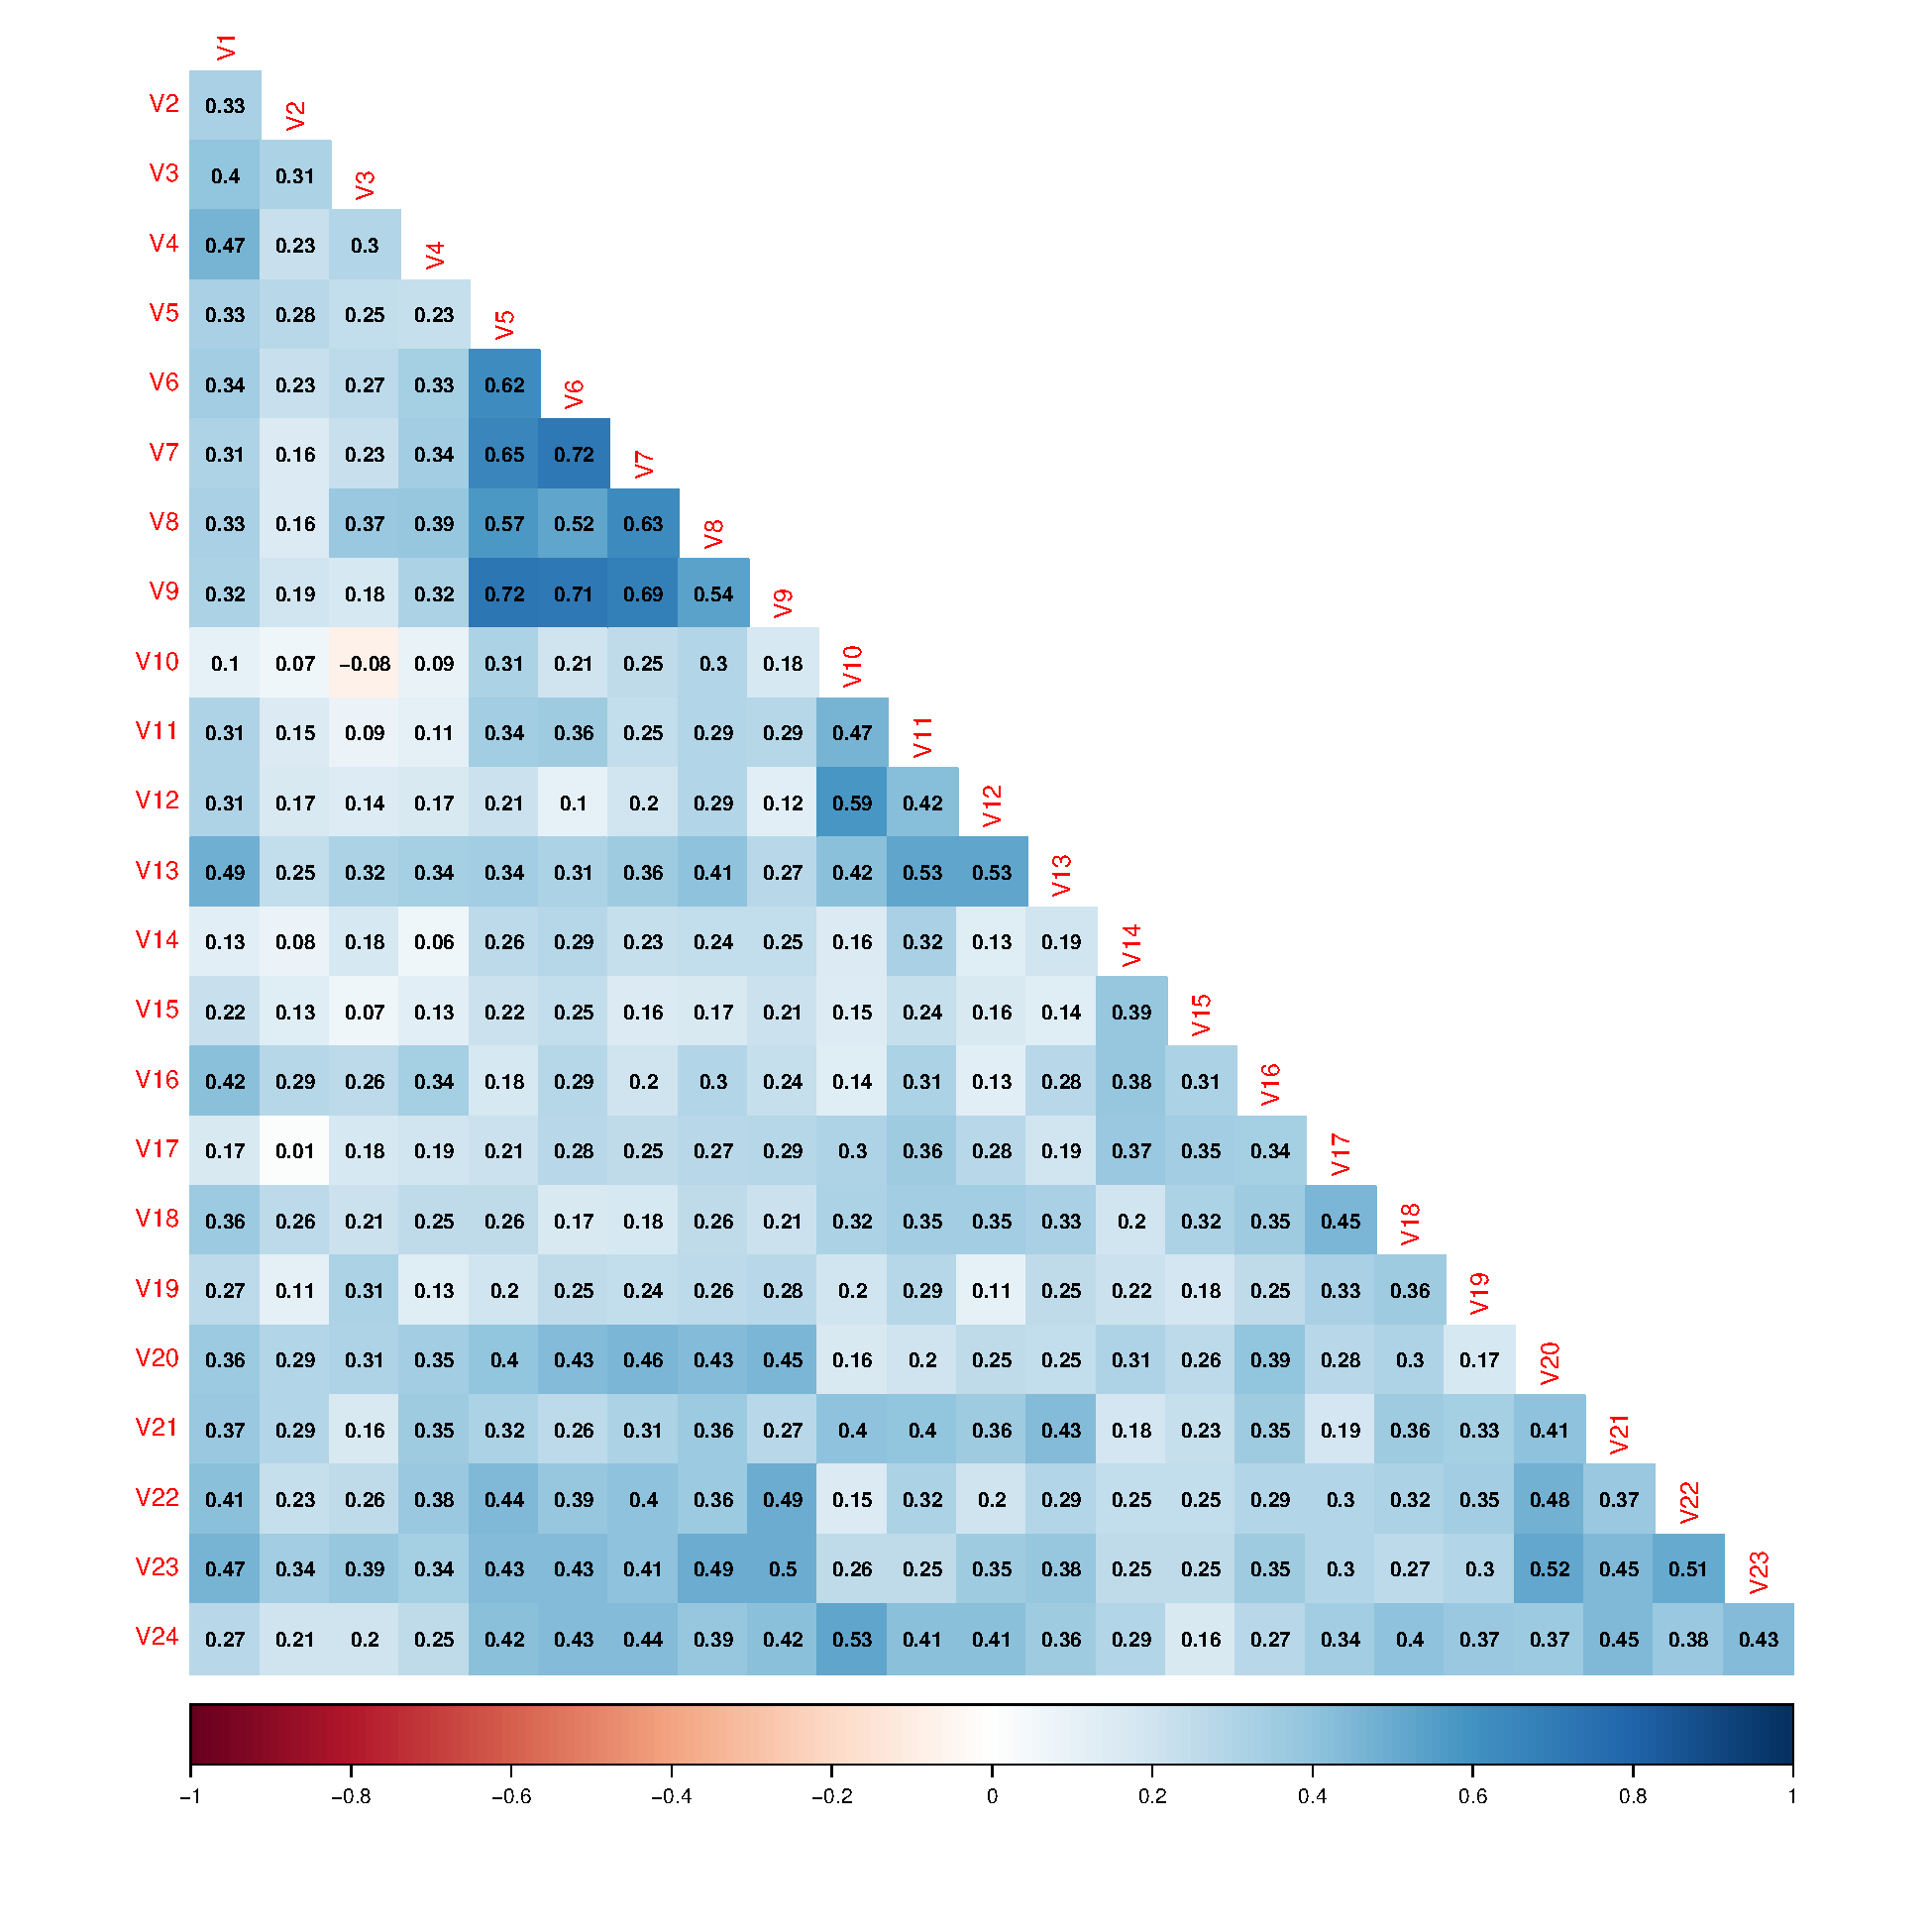
\includegraphics{ProblemSet2_files/figure-pdf/unnamed-chunk-7-1.pdf}

Looking at the plot of the correlations, we can immediately observe the
presence of some groups of quite significantly correlated variables. The
most evident one is composed by the variables \texttt{V5}, \texttt{V6},
\texttt{V7}, \texttt{V8} and \texttt{V9}. Looking at the type of the
tests they represent, we can observe that all those variables are
related to a linguistic or verbal area, hence we do expect them to be
highly correlated, and we may also expect them to be explained by a
common factor.

With a slightly greater level of uncertainty, we can also identify the
group of the variables \texttt{V10}, \texttt{V11}, \texttt{V12} and
\texttt{V13}. In this case the relationship among the variables is less
clear, since we do not know how the tests have been performed and what
they aim to measure. Nevertheless we may think to coding, additions,
counting dots and recognition of capital letters as quite simple tasks
and so we may expect that the students who score higher in these tests
may be the most precise or focused. This may explain why the results of
these tests are quite highly correlated.

Finally, we also mention the group of the variables \texttt{V20},
\texttt{V21}, \texttt{V22}, \texttt{V23} and \texttt{V9} - all quite
related to some logical or problem solving skills.

Overall, we can say that almost the totality of the correlations are
positive and that the majority of them are quite small - or at least
smaller than 0.5.

In particular, we are asked to perform a Factor Analysis with \(m=5\)
and \(m=6\) common factors using the maximum likelihood approach. In R
we can use the command \texttt{factanal}, however in applying this
function we rely on the strong assumption of normality of the data.
Therefore we start by assessing this assumption.

To do so we plot the chi-square qq-plot of the squared Mahalanobis
distances: under the assumption of multivariate normality, the data will
fall along the bisector.

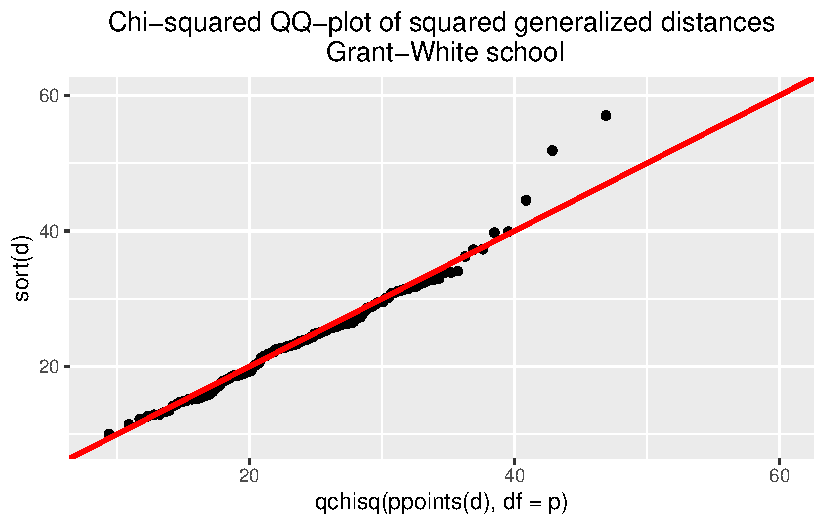
\includegraphics{ProblemSet2_files/figure-pdf/unnamed-chunk-9-1.pdf}

As we can see from the plot, the points deviate from the straight line
only in the right top end. This indicates that the largest values are
more spread out than for a \(\chi_{24}^2\): the tail of the chi-square
distribution is lighter. So, the plot seems to suggest that the
Mahalanobis distances in the sample are more right skewed than you would
expect to see with a multivariate normal.

Nevertheless, we also observe that the points responsible for this
potential non-gaussian behavior are only three, hence they could simply
be multivariate outliers.

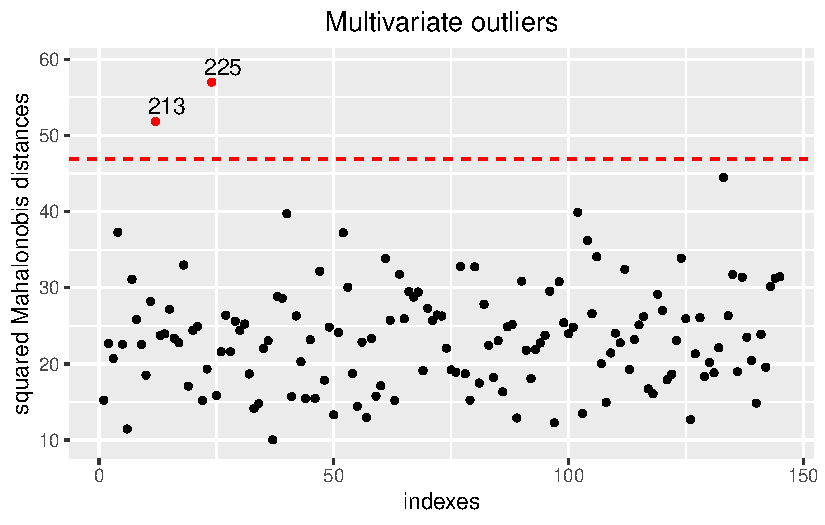
\includegraphics{ProblemSet2_files/figure-pdf/unnamed-chunk-10-1.pdf}

As we can immediately see from the plot, observations having values 213
and 225 of the \texttt{Case} variable - in the original data set - are
multivariate outliers: it is then customary to temporarily remove them
and study again the multivariate normality of the dataset.

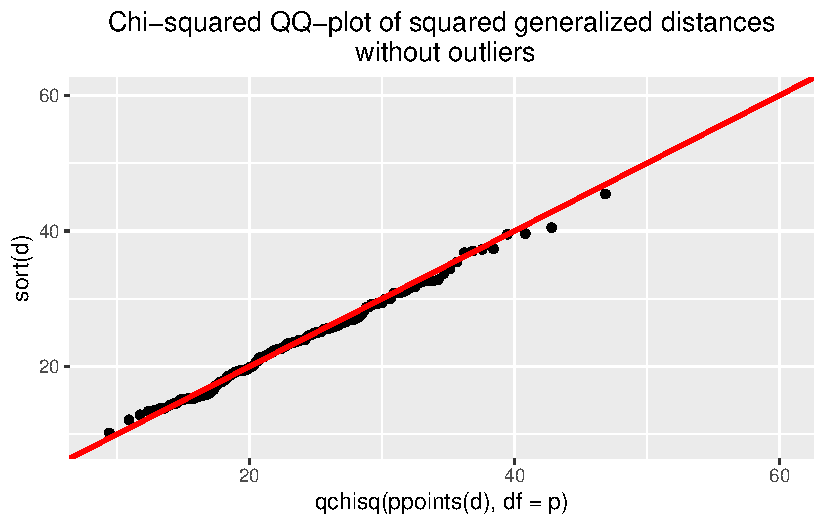
\includegraphics{ProblemSet2_files/figure-pdf/unnamed-chunk-11-1.pdf}

The chi-square qq-plot of the Mahalanobis distances now seems to fit
well the assumption of multivariate normality.

As a final further test, we list the result of the Henze-Zirkler's
multivariate normality test and of the Mardia's multivariate skewness
and kurtosis coefficients as well as their corresponding statistical
significance. The tests are performed using the function \texttt{mvn} in
the \texttt{MVN} package. We test the whole data set:

\begin{verbatim}
           Test        HZ   p value MVN
1 Henze-Zirkler 0.9997837 0.4123569 YES
\end{verbatim}

\begin{verbatim}
             Test        Statistic              p value Result
1 Mardia Skewness 2867.01367856929 0.000163876133958305     NO
2 Mardia Kurtosis 1.24485915986261    0.213183525332604    YES
3             MVN             <NA>                 <NA>     NO
\end{verbatim}

as already highlighted using the chi-square qq-plot, the problem seems
to lie in the skewness of the data. If then we re-do the analysis
without taking into account the outliers:

\begin{verbatim}
           Test        HZ   p value MVN
1 Henze-Zirkler 0.9998182 0.3366856 YES
\end{verbatim}

\begin{verbatim}
             Test          Statistic           p value Result
1 Mardia Skewness   2663.88953618774 0.187254232636786    YES
2 Mardia Kurtosis -0.639916415536184 0.522226941149228    YES
3             MVN               <NA>              <NA>    YES
\end{verbatim}

All problems seem to disappear and multivariate normality can be taken
for granted.

We can now legitimately proceed with the maximum likelihood approach to
perform the Factor Analysis. As requested, we consider and compare the
choices of \(m=5\) and \(m=6\) factors without applying, for now, any
rotation (that we will use later for interpretation purposes).

\begin{Shaded}
\begin{Highlighting}[]
\NormalTok{m }\OtherTok{=} \FunctionTok{c}\NormalTok{(}\DecValTok{5}\NormalTok{,}\DecValTok{6}\NormalTok{)}
\NormalTok{psych}\FloatTok{.5}\NormalTok{fa.ml }\OtherTok{\textless{}{-}} \FunctionTok{factanal}\NormalTok{(}\AttributeTok{x=}\NormalTok{Grant\_White, }\AttributeTok{factors =}\NormalTok{ m[}\DecValTok{1}\NormalTok{], }\AttributeTok{rotation =} \StringTok{"none"}\NormalTok{)}
\NormalTok{psych}\FloatTok{.6}\NormalTok{fa.ml }\OtherTok{\textless{}{-}} \FunctionTok{factanal}\NormalTok{(}\AttributeTok{x=}\NormalTok{Grant\_White, }\AttributeTok{factors =}\NormalTok{ m[}\DecValTok{2}\NormalTok{], }\AttributeTok{rotation =} \StringTok{"none"}\NormalTok{)}
\end{Highlighting}
\end{Shaded}

We start by looking at the obtained loadings, in the case of 5 factors:

\begin{Shaded}
\begin{Highlighting}[]
\NormalTok{L.}\FloatTok{5.}\NormalTok{ml }\OtherTok{\textless{}{-}}\NormalTok{ psych}\FloatTok{.5}\NormalTok{fa.ml}\SpecialCharTok{$}\NormalTok{loadings; L.}\FloatTok{5.}\NormalTok{ml}
\end{Highlighting}
\end{Shaded}

\begin{verbatim}

Loadings:
    Factor1 Factor2 Factor3 Factor4 Factor5
V1   0.555           0.466  -0.150         
V2   0.344           0.292           0.125 
V3   0.373  -0.142   0.427  -0.104         
V4   0.463  -0.104   0.303  -0.113   0.148 
V5   0.723  -0.254  -0.225                 
V6   0.721  -0.374  -0.168          -0.145 
V7   0.728  -0.335  -0.232  -0.132         
V8   0.692  -0.144          -0.107         
V9   0.723  -0.424  -0.197                 
V10  0.518   0.603  -0.379           0.116 
V11  0.570   0.349                  -0.367 
V12  0.487   0.544          -0.118   0.128 
V13  0.631   0.347   0.201  -0.383  -0.206 
V14  0.393                   0.369  -0.238 
V15  0.346           0.128   0.368  -0.128 
V16  0.456           0.378   0.276         
V17  0.453   0.128           0.438  -0.113 
V18  0.475   0.252   0.218   0.259         
V19  0.418           0.138   0.196         
V20  0.596  -0.167   0.181   0.155   0.227 
V21  0.574   0.227   0.154           0.159 
V22  0.595  -0.139   0.180   0.129         
V23  0.665           0.213           0.244 
V24  0.657   0.186  -0.126   0.145   0.129 

               Factor1 Factor2 Factor3 Factor4 Factor5
SS loadings      7.581   1.674   1.316   0.959   0.535
Proportion Var   0.316   0.070   0.055   0.040   0.022
Cumulative Var   0.316   0.386   0.440   0.480   0.503
\end{verbatim}

and of 6:

\begin{Shaded}
\begin{Highlighting}[]
\NormalTok{L.}\FloatTok{6.}\NormalTok{ml }\OtherTok{\textless{}{-}}\NormalTok{ psych}\FloatTok{.6}\NormalTok{fa.ml}\SpecialCharTok{$}\NormalTok{loadings; L.}\FloatTok{6.}\NormalTok{ml}
\end{Highlighting}
\end{Shaded}

\begin{verbatim}

Loadings:
    Factor1 Factor2 Factor3 Factor4 Factor5 Factor6
V1   0.549           0.456  -0.197                 
V2   0.339           0.301  -0.158           0.232 
V3   0.373  -0.139   0.444  -0.111          -0.232 
V4   0.460  -0.107   0.304  -0.133   0.126         
V5   0.724  -0.261  -0.217                         
V6   0.724  -0.367  -0.156          -0.146         
V7   0.733  -0.354  -0.234                  -0.148 
V8   0.695  -0.155          -0.105          -0.207 
V9   0.728  -0.421  -0.180                         
V10  0.513   0.587  -0.385           0.160         
V11  0.579   0.390                  -0.422   0.127 
V12  0.482   0.536          -0.165   0.128  -0.103 
V13  0.618   0.328   0.153  -0.357  -0.228  -0.140 
V14  0.398                   0.353  -0.131         
V15  0.349           0.146   0.332                 
V16  0.457           0.388   0.210                 
V17  0.474   0.180           0.570          -0.257 
V18  0.478   0.278   0.233   0.221                 
V19  0.422           0.154   0.184                 
V20  0.596  -0.156   0.201           0.231         
V21  0.571   0.232   0.151           0.137   0.216 
V22  0.597  -0.121   0.198                   0.169 
V23  0.662           0.229           0.226         
V24  0.656   0.190  -0.113           0.158         

               Factor1 Factor2 Factor3 Factor4 Factor5 Factor6
SS loadings      7.602   1.707   1.351   1.000   0.509   0.419
Proportion Var   0.317   0.071   0.056   0.042   0.021   0.017
Cumulative Var   0.317   0.388   0.444   0.486   0.507   0.525
\end{verbatim}

In particular the proportion of variance explained by each factor is
computed as the sum of the squared loadings of the considered factor
divided by the number of variables \(p=24\). We get the following
results:

\begin{Shaded}
\begin{Highlighting}[]
\NormalTok{L5 }\OtherTok{\textless{}{-}}\NormalTok{ psych}\FloatTok{.5}\NormalTok{fa.ml}\SpecialCharTok{$}\NormalTok{loadings}
\NormalTok{L6 }\OtherTok{\textless{}{-}}\NormalTok{ psych}\FloatTok{.6}\NormalTok{fa.ml}\SpecialCharTok{$}\NormalTok{loadings}

\NormalTok{sL5 }\OtherTok{\textless{}{-}} \FunctionTok{colSums}\NormalTok{(L5}\SpecialCharTok{\^{}}\DecValTok{2}\NormalTok{)}
\NormalTok{sL6 }\OtherTok{\textless{}{-}} \FunctionTok{colSums}\NormalTok{(L6}\SpecialCharTok{\^{}}\DecValTok{2}\NormalTok{)}

\FunctionTok{rbind}\NormalTok{(}\StringTok{\textasciigrave{}}\AttributeTok{Proportion Var}\StringTok{\textasciigrave{}} \OtherTok{=} \FunctionTok{round}\NormalTok{(sL5}\SpecialCharTok{/}\NormalTok{p, 3L))}
\end{Highlighting}
\end{Shaded}

\begin{verbatim}
               Factor1 Factor2 Factor3 Factor4 Factor5
Proportion Var   0.316    0.07   0.055    0.04   0.022
\end{verbatim}

\begin{Shaded}
\begin{Highlighting}[]
\FunctionTok{rbind}\NormalTok{(}\StringTok{\textasciigrave{}}\AttributeTok{Proportion Var}\StringTok{\textasciigrave{}} \OtherTok{=} \FunctionTok{round}\NormalTok{(sL6}\SpecialCharTok{/}\NormalTok{p, 3L))}
\end{Highlighting}
\end{Shaded}

\begin{verbatim}
               Factor1 Factor2 Factor3 Factor4 Factor5 Factor6
Proportion Var   0.317   0.071   0.056   0.042   0.021   0.017
\end{verbatim}

As we have seen in the lectures, the proportion of variance explained by
each factor indicates how much of the total variability of the original
variables is accounted for by that particular factor. Specifically, it
represents the proportion of the total variance in the observed
variables that can be attributed to that factor. For this reason it is
usually used to address the relevance of the factors and, consequently,
as a support to the choice of the number of factors to retain.

As a general guideline we can say that factors that explain a large
proportion of the variance of the original variables are considered more
important and may be more useful for further analysis. Conversely,
factors that explain a small proportion of the variance may be less
useful and can potentially be dropped from further analysis.

Nevertheless it is important to always keep in mind that there is not a
unique way to decide how many factors we should retain. Each situation
need to be analyzed separately and other factors - such as
interpretability and theoretical considerations - may play a relevant
role.

In our situation we can observe that the first factor explains quite a
relevant percentage - the 30\% - of the total variability of the data.
Therefore we expect it to be in some sense the most important of all
factors and to represent an ``important cognitive skill''. The other
factors account for a much smaller proportion. Surely the less
explanatory ones are the fifth and the sixth - when present - factors,
as they respectively explain the 2.2/2.1\% and the 1.7\% of the total
variance. In particular, the fact that they explain a relatively small
but similar proportion of variance seems to suggest that we should
reserve the same treatment to both of them - i.e.~retain or discard them
both. However, as said before, the decision to discard a factor should
not be based solely on the proportion of variance it explains, hence
before making any further consideration we proceed in our analysis.

Given the proportion of variance accounted for by each factor, we can
also compute the cumulative proportion of variance explained by the
\(m\) factors. To do so we simply apply the function \texttt{cumsum} to
the single proportion of variances.

\begin{Shaded}
\begin{Highlighting}[]
\FunctionTok{rbind}\NormalTok{(}\StringTok{\textasciigrave{}}\AttributeTok{Cumulative Var}\StringTok{\textasciigrave{}} \OtherTok{=} \FunctionTok{round}\NormalTok{(}\FunctionTok{cumsum}\NormalTok{(sL5}\SpecialCharTok{/}\NormalTok{p), 3L))}
\end{Highlighting}
\end{Shaded}

\begin{verbatim}
               Factor1 Factor2 Factor3 Factor4 Factor5
Cumulative Var   0.316   0.386    0.44    0.48   0.503
\end{verbatim}

\begin{Shaded}
\begin{Highlighting}[]
\FunctionTok{rbind}\NormalTok{(}\StringTok{\textasciigrave{}}\AttributeTok{Cumulative Var}\StringTok{\textasciigrave{}} \OtherTok{=} \FunctionTok{round}\NormalTok{(}\FunctionTok{cumsum}\NormalTok{(sL6}\SpecialCharTok{/}\NormalTok{p), 3L))}
\end{Highlighting}
\end{Shaded}

\begin{verbatim}
               Factor1 Factor2 Factor3 Factor4 Factor5 Factor6
Cumulative Var   0.317   0.388   0.444   0.486   0.507   0.525
\end{verbatim}

As we can see, both the factor analysis performed with 5 factors and the
one with 6 factors only explain slightly more than the 50\% of the total
variability of the data. Therefore, they don't seem to be a good fit for
the data.

Now, in a real-life study, there are several things we can do to try
improve the fit of the model, some examples include:

\begin{itemize}
\tightlist
\item
  removing the outliers from the data set and re-estimate the maximum
  likelihood solution;
\item
  using different methods to perform the factor analysis - for example a
  possibility is to use the principal component approach;
\item
  finally, we may consider alternative analyses - such as principal
  component analysis, cluster analysis, or discriminant analysis.
\end{itemize}

We will not try any of these improvement, but - for the sake of the
exercise - we will proceed in the factor analysis taking this issue into
account.

Other relevant features to examine are the specific variances, or
uniquenesses. The \(i^{th}\) uniqueness represents the proportion of
variance of the \(i^{th}\) variable that is not accounted for by the
factors. In other words, the specific variances are important because
they provide information about the unique contribution of each observed
variable to the total variance. Variables with large specific variances
are those that are not well accounted for by the underlying factors.
These variables are also more likely to have weaker factor loadings and
may be more difficult to interpret. On the other hand, variables with
small specific variances are those that are well explained by the
factors and are more likely to have stronger factor loadings.

For all these reasons, the specific variances can also affect the
decision of how many factors to retain in the analysis: if there are
many observed variables with high specific variances, this may indicate
the necessity to add some extra factors.

The specific variances can also be used to assess the overall fit of the
factor model. If the specific variances are very large, this may
indicate that the model is not a good fit for the data and may need to
be modified Alternatively, if the specific variances are very small,
this may indicate that the model is over-fitting the data and may need
to be simplified.

Overall, specific variances are an important part of the output of
factor analysis and can provide valuable information about the quality
of the factor model and the interpretation of the results.

We list our results:

\begin{verbatim}
    uniquenesses_nfactors_5 uniquenesses_nfactors_6
V1                    0.453                   0.447
V2                    0.777                   0.710
V3                    0.646                   0.577
V4                    0.648                   0.643
V5                    0.357                   0.346
V6                    0.291                   0.295
V7                    0.286                   0.252
V8                    0.481                   0.429
V9                    0.257                   0.248
V10                   0.208                   0.216
V11                   0.413                   0.311
V12                   0.436                   0.426
V13                   0.253                   0.289
V14                   0.649                   0.693
V15                   0.712                   0.732
V16                   0.565                   0.586
V17                   0.572                   0.347
V18                   0.596                   0.586
V19                   0.761                   0.758
V20                   0.509                   0.513
V21                   0.569                   0.523
V22                   0.568                   0.549
V23                   0.447                   0.449
V24                   0.480                   0.485
\end{verbatim}

As we could expect from the fact that the total variance explained by
the common factors is quite low, the uniquenesses are generally quite
high. Moreover, there are no variables with a specific variance that can
be considered particularly small: the variable that is best explained by
the factors has a uniqueness greater than 0.2.

We are mainly interested in two different aspects:

\begin{itemize}
\tightlist
\item
  high specific variances (or very low ones, but there isn't any in our
  case);
\item
  significant difference among the uniquenesses returned using 5 or 6
  factors.
\end{itemize}

For what concern the higher specific variances, we can observe that
there are 16 variables for which the uniquenesses in both cases are -
for example - higher than 0.4, specifically:

\begin{verbatim}
    uniquenesses_nfactors_5 uniquenesses_nfactors_6
V1                    0.453                   0.447
V2                    0.777                   0.710
V3                    0.646                   0.577
V4                    0.648                   0.643
V8                    0.481                   0.429
V12                   0.436                   0.426
V14                   0.649                   0.693
V15                   0.712                   0.732
V16                   0.565                   0.586
V18                   0.596                   0.586
V19                   0.761                   0.758
V20                   0.509                   0.513
V21                   0.569                   0.523
V22                   0.568                   0.549
V23                   0.447                   0.449
V24                   0.480                   0.485
\end{verbatim}

Again, the presence of such a great number of variables with high
uniquenesses may suggests that the model does not fit the data very
well.

Keeping this in mind, it is also important to note that high uniqueness
values are not necessarily a problem in themselves. Some variables will
naturally have higher uniqueness values than others, depending on their
level of specificity or measurement precision. Therefore one should
always consider the specific context of the phenomenon being studied.

In our analysis, the presence of such a high number of variables with
high uniqueness value may not be completely unexpected: the data are
related to aptitude tests on students, thus it seems reasonable to
expect that the tests also rely heavily on individual abilities of
pupils that the common factor would fail to encode.

Nevertheless, the number of factors with a great amount of unexplained
variability seems to us too high to be ignored, even if we keep into
account the individual characteristics of the students.

Let's now look at the variables for which the inclusion of the sixth
factors plays a relevant role.

In particular we decided to print the specific variances of the
variables for which the addition of the sixth factor lead to a decrease
- or increase - of the specific variance greater than 0.1. We also
return them in decreasing order: the first variable returned is the one
with the greatest gap among the two uniquenesses.

\begin{verbatim}
    uniquenesses_nfactors_5 uniquenesses_nfactors_6
V17                   0.572                   0.347
V11                   0.413                   0.311
\end{verbatim}

As we can observe, the variables that are mainly affected by the
introduction of a new factor are \texttt{V17} - an object-number test -
and \texttt{V11} - a code-test. So we expect these two variables to be
better explained by 6 common factors than 5.

It is also worth noticing that the number of variables for which the
uniquenesses are significantly reduced by the introduction of the sixth
factor is only two. This may suggest that the model with 6 factors may
fail in providing a relevant improvement with respect to the one with 5
factors.

We can now assess the approximation of the correlation matrix. To do so
we can compute the residual matrix \[
\begin{aligned}
  \mathbf{R} - \hat{\mathbf{L}}\hat{\mathbf{L}}^T - \hat{\mathbf{\Psi}}
\end{aligned}
\]

resulting from the approximation of \(\mathbf{R}\) via the simpler
structure \(\hat{\mathbf{L}}\hat{\mathbf{L}}^T + \hat{\mathbf{\Psi}}\).
We can then summarize how far from the perfect approximation we are by
computing its Frobenius norm.

\begin{Shaded}
\begin{Highlighting}[]
\NormalTok{Psi.}\FloatTok{5.}\NormalTok{ml }\OtherTok{\textless{}{-}} \FunctionTok{diag}\NormalTok{(psych}\FloatTok{.5}\NormalTok{fa.ml}\SpecialCharTok{$}\NormalTok{uniquenesses, p)}
\NormalTok{Psi.}\FloatTok{6.}\NormalTok{ml }\OtherTok{\textless{}{-}} \FunctionTok{diag}\NormalTok{(psych}\FloatTok{.6}\NormalTok{fa.ml}\SpecialCharTok{$}\NormalTok{uniquenesses, p)}

\NormalTok{Residual.}\FloatTok{5.}\NormalTok{ml }\OtherTok{\textless{}{-}}\NormalTok{ R }\SpecialCharTok{{-}}\NormalTok{ (L.}\FloatTok{5.}\NormalTok{ml}\SpecialCharTok{\%*\%}\FunctionTok{t}\NormalTok{(L.}\FloatTok{5.}\NormalTok{ml) }\SpecialCharTok{+}\NormalTok{ Psi.}\FloatTok{5.}\NormalTok{ml)}
\NormalTok{Residual.}\FloatTok{6.}\NormalTok{ml }\OtherTok{\textless{}{-}}\NormalTok{ R }\SpecialCharTok{{-}}\NormalTok{ (L.}\FloatTok{6.}\NormalTok{ml}\SpecialCharTok{\%*\%}\FunctionTok{t}\NormalTok{(L.}\FloatTok{6.}\NormalTok{ml) }\SpecialCharTok{+}\NormalTok{ Psi.}\FloatTok{6.}\NormalTok{ml)}

\NormalTok{Frob.res }\OtherTok{\textless{}{-}} \FunctionTok{cbind}\NormalTok{(}\FunctionTok{sum}\NormalTok{(Residual.}\FloatTok{5.}\NormalTok{ml}\SpecialCharTok{\^{}}\DecValTok{2}\NormalTok{), }\FunctionTok{sum}\NormalTok{(Residual.}\FloatTok{6.}\NormalTok{ml}\SpecialCharTok{\^{}}\DecValTok{2}\NormalTok{))}

\FunctionTok{row.names}\NormalTok{(Frob.res) }\OtherTok{\textless{}{-}} \StringTok{"Frobenius norm of the residual matrix: "}
\FunctionTok{colnames}\NormalTok{(Frob.res) }\OtherTok{\textless{}{-}} \FunctionTok{c}\NormalTok{(}\StringTok{"nFactors\_5"}\NormalTok{, }\StringTok{"nFactors\_6"}\NormalTok{)}

\FunctionTok{as.data.frame}\NormalTok{(}\FunctionTok{round}\NormalTok{(Frob.res, }\DecValTok{3}\NormalTok{))}
\end{Highlighting}
\end{Shaded}

\begin{verbatim}
                                        nFactors_5 nFactors_6
Frobenius norm of the residual matrix:       0.734      0.602
\end{verbatim}

The obtained norms - for the choice of 5 and 6 factors - are in both
cases quite high, even if adding the sixth factor slightly reduces it.
This may again be explained by keeping into account the fact that in
both cases the total cumulative variance explained by the factors is
quite small - 0.503 and 0.525 respectively. Therefore, we can conclude
that, despite the improvement in the approximation related to the
inclusion of the sixth factor, in both cases the approximation of the
correlation matrix is not so satisfactory.

Overall, the comparison seems to suggests that neither the 5 factors
model nor the 6 factors one are good fit for the data. Anyway, if we
stick to the problem of deciding how many factors to retain, the choice
of 5 common factors may appear to be the preferable one. Indeed, as it
emerges from all the comments above, the improvements related to the use
of six factors are not sufficiently noteworthy.

\hypertarget{give-an-interpretation-to-the-common-factors-in-the-m-5-solution-with-varimax-rotation}{%
\subsubsection{\texorpdfstring{2. Give an interpretation to the common
factors in the \(m = 5\) solution with varimax
rotation}{2. Give an interpretation to the common factors in the m = 5 solution with varimax rotation}}\label{give-an-interpretation-to-the-common-factors-in-the-m-5-solution-with-varimax-rotation}}

To give an easier interpretation of the factors, we can perform a
varimax rotation. The varimax technique seeks the rotated loadings
\(\mathbf{L}^*\) that maximize the variance of the squared loadings for
each factor. Loosely speaking, this maximization has the effect of
``spreading out'' the squares of the loadings on each factor as much as
possible. In other words, the varimax rotation technique attempts to
make the loadings either small or large to facilitate interpretation.
Therefore performing a varimax rotation aims to find groups of large and
the negligible in each column of the rotated loadings matrix
\(\mathbf{L}^*\).

\begin{Shaded}
\begin{Highlighting}[]
\NormalTok{psych}\FloatTok{.5}\NormalTok{fa.ml }\OtherTok{\textless{}{-}} \FunctionTok{factanal}\NormalTok{(}\AttributeTok{x=}\NormalTok{Grant\_White, }\AttributeTok{factors =}\NormalTok{ m[}\DecValTok{1}\NormalTok{], }\AttributeTok{rotation =} \StringTok{"varimax"}\NormalTok{)}
\NormalTok{psych}\FloatTok{.5}\NormalTok{fa.ml}\SpecialCharTok{$}\NormalTok{loadings}
\end{Highlighting}
\end{Shaded}

\begin{verbatim}

Loadings:
    Factor1 Factor2 Factor3 Factor4 Factor5
V1   0.165   0.655   0.125   0.181   0.207 
V2   0.108   0.442                         
V3   0.134   0.559           0.112         
V4   0.230   0.533                         
V5   0.738   0.189   0.192   0.149         
V6   0.772   0.187           0.248   0.124 
V7   0.798   0.214   0.143                 
V8   0.571   0.343   0.239   0.128         
V9   0.808   0.202           0.219         
V10  0.181  -0.108   0.845   0.180         
V11  0.195           0.423   0.436   0.418 
V12          0.232   0.694   0.102   0.129 
V13  0.186   0.433   0.479           0.538 
V14  0.185                   0.552         
V15  0.104   0.122           0.509         
V16          0.406           0.509         
V17  0.154           0.210   0.595         
V18          0.300   0.322   0.458         
V19  0.156   0.221   0.144   0.378         
V20  0.373   0.461   0.127   0.293  -0.194 
V21  0.172   0.398   0.431   0.238         
V22  0.364   0.423   0.114   0.320         
V23  0.362   0.542   0.248   0.231  -0.115 
V24  0.368   0.179   0.495   0.321         

               Factor1 Factor2 Factor3 Factor4 Factor5
SS loadings      3.640   2.957   2.454   2.386   0.628
Proportion Var   0.152   0.123   0.102   0.099   0.026
Cumulative Var   0.152   0.275   0.377   0.477   0.503
\end{verbatim}

Before proceeding with the interpretation it is worth noticing that the
fifth factor explains a proportion of variance that is much smaller than
the other four. Thus we expect it to be the most difficult to interpret.

In order to interpret the factors we classify the observed variables
into five groups - each one corresponding to a different factor - based
on their loadings.

As a first subdivision we simply choose to assign each variable to the
factor corresponding to its greatest loading. Then we assess the
significance of the loadings using a threshold value equal to 0.5.

The group of variables associated to the first factor is given by:

\begin{verbatim}
  var                 meaning load.max
1  V5     general information    0.738
2  V6 paragraph comprehension    0.772
3  V7     sentence completion    0.798
4  V8     word classification    0.571
5  V9            word meaning    0.808
\end{verbatim}

We can immediately notice that the considered loadings of all the
variables in this group have a high enough level of significance.

The interpretation of this factor seems also quite straightforward, as
all the variables associated to it are related to some kind of
linguistic and comprehension abilities. The tests indeed are devised to
target students capacity to understand the meaning of a phrase or a word
as well as their aptitude to correctly identify the class of a word or
complete a sentence.

For this reason we may denote it as ``verbal intelligence''.

The group of variables associated to the second factor is:

\begin{verbatim}
  var           meaning load.max
1  V1 visual perception    0.655
2  V2             cubes    0.442
3  V3  paper form board    0.559
4  V4             flags    0.533
5 V20         deduction    0.461
6 V22 problem reasoning    0.423
7 V23 series completion    0.542
\end{verbatim}

Based on our significance threshold value, only the following four
variables should be retained:

\begin{verbatim}
  var           meaning load.max
1  V1 visual perception    0.655
2  V3  paper form board    0.559
3  V4             flags    0.533
4 V23 series completion    0.542
\end{verbatim}

The variables \texttt{V1}-\texttt{V3}-\texttt{V4} seem to be related to
the ability to deal with spatial and visual relations or, more
precisely, to the ability of an individual to visualize and manipulate
objects in space. These capacities surely play also a relevant role in
determining one's skill to complete a given series. However, the results
of the \(23^{th}\) test is necessarily also connected to some
problem-solving and logical capabilities, as it requires some imagery
capacity, mental visualization skills and part-whole relationship
skills.

If we also look at the excluded variables - \texttt{V2}, \texttt{V20},
\texttt{V22} - all seems to be in some sense related to the already
identified visual, spatial and logical spheres. This give further
support to our interpretation.

Consequently, we can call this factor ``visual,spatial and logic
intelligence''.

The group of variables associated to the third factor is:

\begin{verbatim}
  var             meaning load.max
1 V10            addition    0.845
2 V12       counting dots    0.694
3 V21   numerical puzzles    0.431
4 V24 arithmetic problems    0.495
\end{verbatim}

Even for this factor there is one variable that we do not consider
significant, \texttt{V21} - actually, we have rounded up the loading of
\texttt{V24}. So the variables to be considered are:

\begin{verbatim}
  var             meaning load.max
1 V10            addition    0.845
2 V12       counting dots    0.694
3 V24 arithmetic problems    0.495
\end{verbatim}

Looking at this group - and also taking into account the fact that the
variable \texttt{V10} represents an addition test and loads highly on
the considered third factor - we may interpret this factor as an
``arithmetic intelligence''.

For what concerns the excluded variable \texttt{V21}, it corresponds to
a numerical-puzzle test and therefore fits quite well in the group
associated with an ``arithmetic intelligence'' factor.

The group of variables associated to the fourth factor is:

\begin{verbatim}
  var            meaning load.max
1 V11               code    0.436
2 V14   word recognition    0.552
3 V15 number recognition    0.509
4 V16 figure recognition    0.509
5 V17      object-number    0.595
6 V18      number-figure    0.458
7 V19        figure-word    0.378
\end{verbatim}

We remove the three variables whose loadings are not significant enough:

\begin{verbatim}
  var            meaning load.max
1 V14   word recognition    0.552
2 V15 number recognition    0.509
3 V16 figure recognition    0.509
4 V17      object-number    0.595
\end{verbatim}

All the variables that load high on the fourth factor are related to the
spheres of recognition and association. Thus this factor may be simply
called ``recognition''.

Once again the excluded variables may be well explained by the
``recognition'' fourth rotated factor.

Finally, the group of variables associated to the fifth factor is:

\begin{verbatim}
  var                  meaning load.max
1 V13 straight-curved capitals    0.538
\end{verbatim}

This group is made of a unique variable, \texttt{V13}, corresponding to
a test involving straight and curved uppercase letters. The factor may
be called ``letter recognition'', but is actually of low relevance.

We can now deal with the variables with an ``ambiguous'' classification.

In particular, the variables for which we have identified some issues
are the following:

\begin{verbatim}
    Factor1 Factor2 Factor3 Factor4 Factor5             meaning
V2    0.108   0.442   0.087   0.095   0.002               cubes
V11   0.195   0.066   0.423   0.436   0.418                code
V18   0.032   0.300   0.322   0.458   0.004       number-figure
V19   0.156   0.221   0.144   0.378   0.045         figure-word
V20   0.373   0.461   0.127   0.293  -0.194           deduction
V21   0.172   0.398   0.431   0.238   0.000   numerical puzzles
V22   0.364   0.423   0.114   0.320  -0.069   problem reasoning
V24   0.368   0.179   0.495   0.321  -0.068 arithmetic problems
\end{verbatim}

As we can see, \texttt{V2} may properly be associated with the second
group, indeed its second factor loading is much greater than all the
others. For the same reason the variables \texttt{V18}, \texttt{V19},
\texttt{V20} and \texttt{V24} may be reasonably added to groups 4, 4, 2
and 3 respectively. So, with the only exceptions of variables
\texttt{V11} and \texttt{V22}, our previous identification of the groups
seems to be quite satisfactory, especially if we consider the fact that
the proportion of cumulative variance explained by the 5 considered
common factors is only equal to the 50\% of the total variability of the
data.

For what concerns the variable \texttt{V11}, we can notice that its
three highest loadings - corresponding to factors 3, 4 and 5 - are all
very similar. This may be reasonable, indeed to score high in a code
test it in necessary not only to have good ``matching'' capacities
(factor 4), but also some mathematical-problem solving skills (factor 3)
and the ability to recognize quickly the elements to code (factor 5).

Similarly, for variable \texttt{V22} we cannot ignore the loading
associated to factor 1, besides the higher one being the one of factor
2. Also in this case, we may interpret this result by saying that
``problem reasoning'' abilities are quite transversal skills and are
surely also related to the verbal sphere.

\hypertarget{make-a-scatterplot-of-the-first-two-factor-scores-for-the-m-5-solution-obtained-by-the-regression-method.-is-their-correlation-equal-to-zero-should-we-expect-so-comment.}{%
\subsubsection{\texorpdfstring{3. Make a scatterplot of the first two
factor scores for the \(m = 5\) solution obtained by the regression
method. Is their correlation equal to zero? Should we expect so?
Comment.}{3. Make a scatterplot of the first two factor scores for the m = 5 solution obtained by the regression method. Is their correlation equal to zero? Should we expect so? Comment.}}\label{make-a-scatterplot-of-the-first-two-factor-scores-for-the-m-5-solution-obtained-by-the-regression-method.-is-their-correlation-equal-to-zero-should-we-expect-so-comment.}}

First of all we make some theoretical observations on the factor scores.

The factor scores are the estimated values of the underlying common
factors. In particular, they are estimates of the unobserved vector
\(f_i = (f_{i1}, \dots, f_{im})\) - in place of which we have only
observed the variables realizations \(x_i = (x_{i1}, \dots, x_{im})\).
The estimation, however, is not straightforward, as the total number of
unobserved quantities - given not only by the \(f_i\), but also by the
error terms \(\epsilon_i\) - outnumbers the observed \(x_i\).

One of the most used approaches advanced to overcome this problem is the
\emph{regression method}. The idea is the following: consider the
baseline equation of the factor model \[
  X - \mu = \mathbf{L}F + \epsilon
\] where we suppose that both the factors and the errors are jointly
normally distributed and that both the common factors and the errors are
uncorrelated within each other. Under these assumption we know that the
conditional distribution of \(F|X\) is again Gaussian, with conditional
mean given by \[
 \mathbf{L}^T\mathbf{\Sigma}^{-1}(X-\mu) = \mathbf{L}^T(\mathbf{LL}^T -\mathbf{\Psi})^{-1}(X-\mu)
\] Given so, a natural estimate for \(f_i\) is simply the corresponding
estimate of this conditional mean: \[
\hat{f_i} = \hat{\mathbf{L}}^T\mathbf{S}^{-1}(x_i-\bar{x})
\] where we use \(\mathbf{S}\) in place of its estimation in order to
try to reduce the effects of possible mistakes in determining the number
of factors.

Given so, since we assume that the common factors are uncorrelated -
\(cov(F_i, F_j) = 0, \quad \forall i\neq j\) - we will get - or at least
we would like to get - uncorrelated factor scores.

We therefore expect that the first and second factor scores are
essentially uncorrelated.

To test our hypothesis we make a scatter plot of the first two factor
scores:

\begin{Shaded}
\begin{Highlighting}[]
\NormalTok{psych}\FloatTok{.5}\NormalTok{fa.ml }\OtherTok{\textless{}{-}} \FunctionTok{factanal}\NormalTok{(}\AttributeTok{x=}\NormalTok{Grant\_White, }\AttributeTok{factors =}\NormalTok{ m[}\DecValTok{1}\NormalTok{], }\AttributeTok{rotation =} \StringTok{"varimax"}\NormalTok{,}
\AttributeTok{scores =} \StringTok{"regression"}\NormalTok{)}
\NormalTok{scores\_GrWh }\OtherTok{\textless{}{-}}\NormalTok{ psych}\FloatTok{.5}\NormalTok{fa.ml}\SpecialCharTok{$}\NormalTok{scores}
\end{Highlighting}
\end{Shaded}

\begin{Shaded}
\begin{Highlighting}[]
\FunctionTok{ggplot}\NormalTok{(}\FunctionTok{as.data.frame}\NormalTok{(scores\_GrWh), }\FunctionTok{aes}\NormalTok{(}\AttributeTok{x =}\NormalTok{ Factor1, }\AttributeTok{y =}\NormalTok{ Factor2)) }\SpecialCharTok{+} 
  \FunctionTok{geom\_point}\NormalTok{() }\SpecialCharTok{+}
  \FunctionTok{ggtitle}\NormalTok{(}\StringTok{"Scatter{-}plot of the first two factor scores}\SpecialCharTok{\textbackslash{}n}\StringTok{ for the Grant{-}White students"}\NormalTok{) }\SpecialCharTok{+}
  \FunctionTok{theme}\NormalTok{(}\AttributeTok{plot.title =} \FunctionTok{element\_text}\NormalTok{(}\AttributeTok{hjust =} \FloatTok{0.5}\NormalTok{, }\AttributeTok{size =} \DecValTok{10}\NormalTok{))}
\end{Highlighting}
\end{Shaded}

\begin{figure}[H]

{\centering 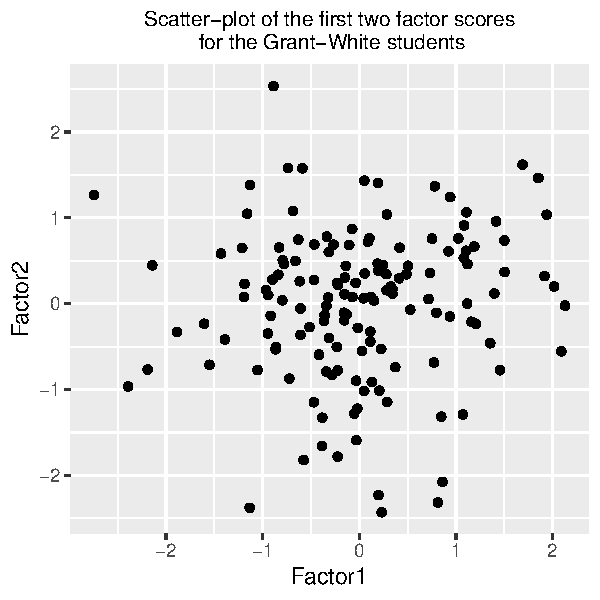
\includegraphics{ProblemSet2_files/figure-pdf/unnamed-chunk-35-1.pdf}

}

\end{figure}

As expected, no clear pattern arises from the scatter plot, suggesting
that the first two factor scores are almost uncorrelated within each
other. Moreover, a numerical computation of the correlation returns:

\begin{verbatim}
  correlation
1  0.07425218
\end{verbatim}

A value that is indeed small.

Finally, a further insightful thing to verify is whether the assumption
of bivariate normality actually holds: in particular, by the theory we
expect that the first and second factors are jointly normally
distributed with mean zero and identity covariance matrix. This is
translated in a plot in which the points are centered around the origin
and the elliptic contour plots have a nice circular shape.

Let's first of all compute the sample means of the two factor scores:

\begin{verbatim}
                     x_bar        y_bar
Grant-White: -6.795331e-18 3.298966e-18
\end{verbatim}

Before plotting the data, we also notice that together with the
assumption of normality, it is important to study the presence of
bivariate outliers. Indeed, outliers can influence the strength and
direction of the correlation. The reason is that outliers can create a
distorted picture of the relationship between the two variables. Thus,
if an outlier is included in a dataset, it can pull the correlation
coefficient in one direction or another, making it appear stronger or
weaker than it actually is, or even falsify the normality assumption.

In our situation, the correlation coefficient is already very low,
therefore we do not expect to find bivariate outliers that are extreme
observations for both observations. For the same reason, we also expect
to find circular contour plots. The ellipses shown in the plot are fit
to the data assuming a Gaussian distribution.

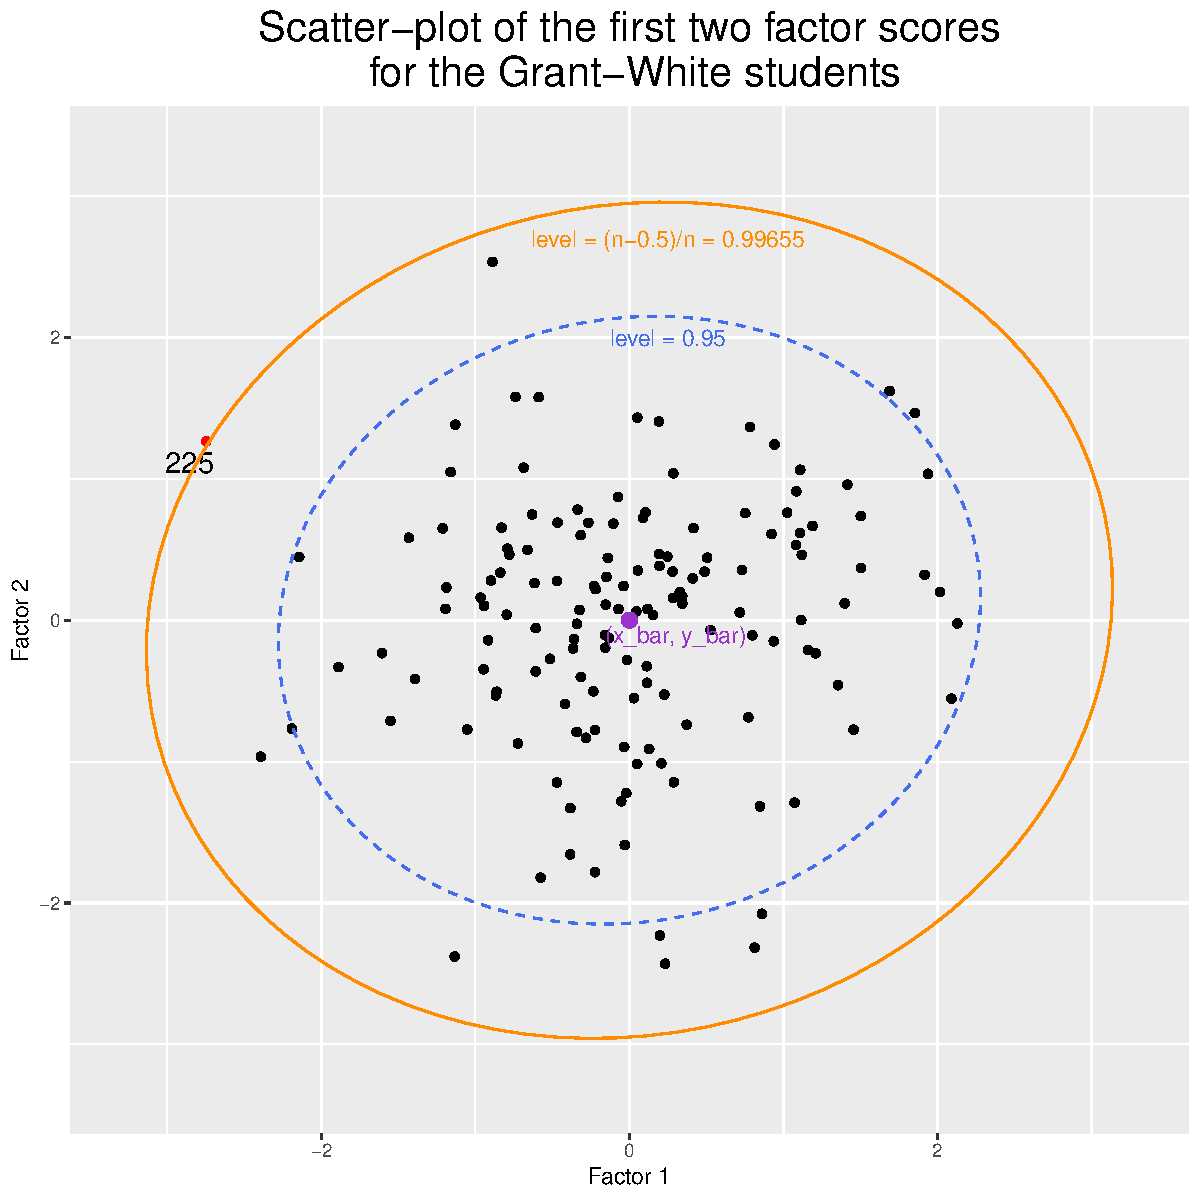
\includegraphics{ProblemSet2_files/figure-pdf/unnamed-chunk-38-1.pdf}

As expected, the desired assumption of normality appears to hold. Indeed
the shape of the bivariate distribution of the first two scores well
resemble a standard bi-dimensional Gaussian. We also notice the presence
of one bivariate outlier that has been identified by means of the
variable \texttt{Case} in the original data set.

\hypertarget{obtain-the-maximum-likelihood-solution-with-varimax-rotation-for-m-5-factors-by-using-the-pasteur-students-data.-is-the-interpretation-to-the-common-factors-similar-to-that-of-grantwhite-students}{%
\subsubsection{\texorpdfstring{4. Obtain the maximum likelihood solution
with varimax rotation for \(m = 5\) factors by using the Pasteur
students data. Is the interpretation to the common factors similar to
that of Grant--White
students?}{4. Obtain the maximum likelihood solution with varimax rotation for m = 5 factors by using the Pasteur students data. Is the interpretation to the common factors similar to that of Grant--White students?}}\label{obtain-the-maximum-likelihood-solution-with-varimax-rotation-for-m-5-factors-by-using-the-pasteur-students-data.-is-the-interpretation-to-the-common-factors-similar-to-that-of-grantwhite-students}}

As requested we now compute the maximum likelihood solution with 5
factors using the data on the students attending the Pasteur school. As
before we only consider the variables related to the 24 attitudinal
tests.

\begin{Shaded}
\begin{Highlighting}[]
\NormalTok{Pasteur }\OtherTok{\textless{}{-}}\NormalTok{ psych }\SpecialCharTok{\%\textgreater{}\%}\NormalTok{ dplyr}\SpecialCharTok{::}\FunctionTok{filter}\NormalTok{(group }\SpecialCharTok{==} \StringTok{"PASTEUR"}\NormalTok{) }\SpecialCharTok{\%\textgreater{}\%}
\NormalTok{dplyr}\SpecialCharTok{::}\FunctionTok{select}\NormalTok{(}\SpecialCharTok{{-}}\FunctionTok{c}\NormalTok{(Case, Sex, Age, group))}
\end{Highlighting}
\end{Shaded}

Let's first of all look at the correlations among those variables.

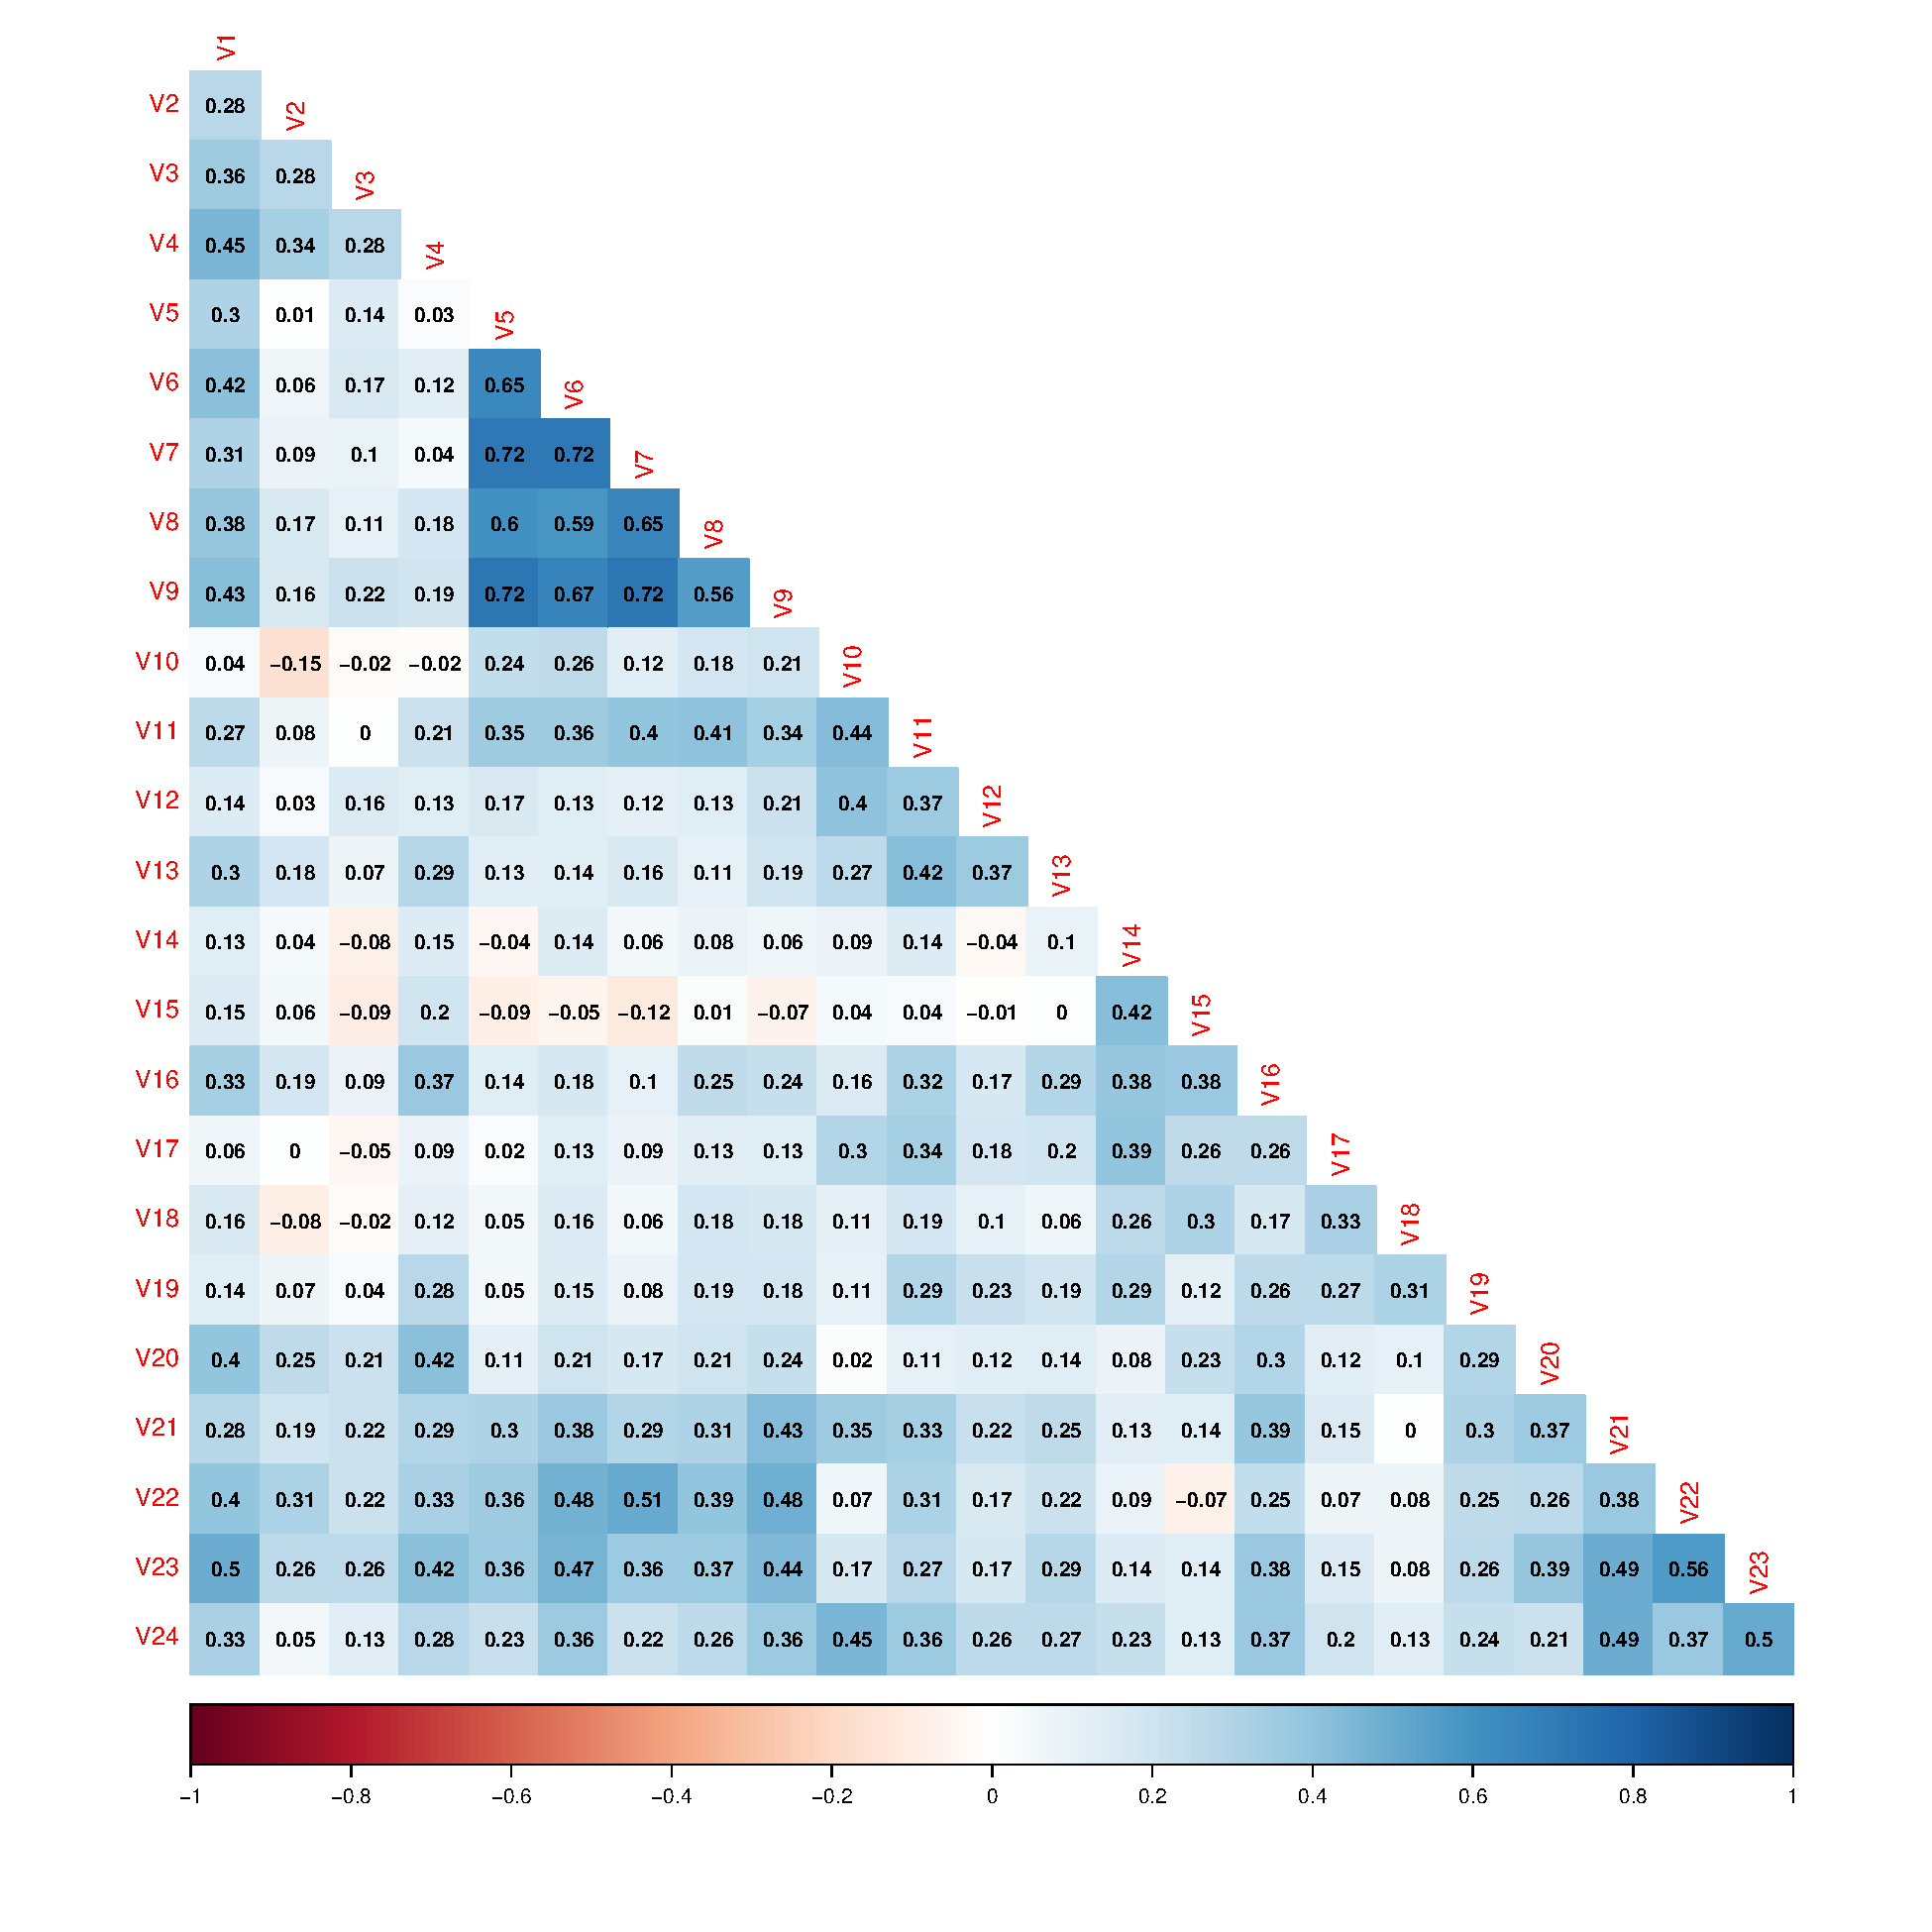
\includegraphics{ProblemSet2_files/figure-pdf/unnamed-chunk-41-1.pdf}

As happened for the data related to the Grant-White school, we can
observe that there is a group of high correlated data corresponding to
variables \texttt{V5}, \texttt{V6}, \texttt{V7}, \texttt{V8} and
\texttt{V9}. This, again, may suggest the existence of an underlying
factor which all those variable refer to. Those variables are also quite
correlated with \texttt{V21}, \texttt{V22} and \texttt{V23}. Finally
some other less clear correlation patterns appear among the variables
\texttt{V10}, \texttt{V11}, \texttt{V12} and \texttt{V13} and maybe also
among \texttt{V14}, \texttt{V15} and \texttt{V16}.

Overall, however, the great majority of correlation coefficients are
quite small and almost all positive.

We also quickly assess the assumption of multivariate normality:

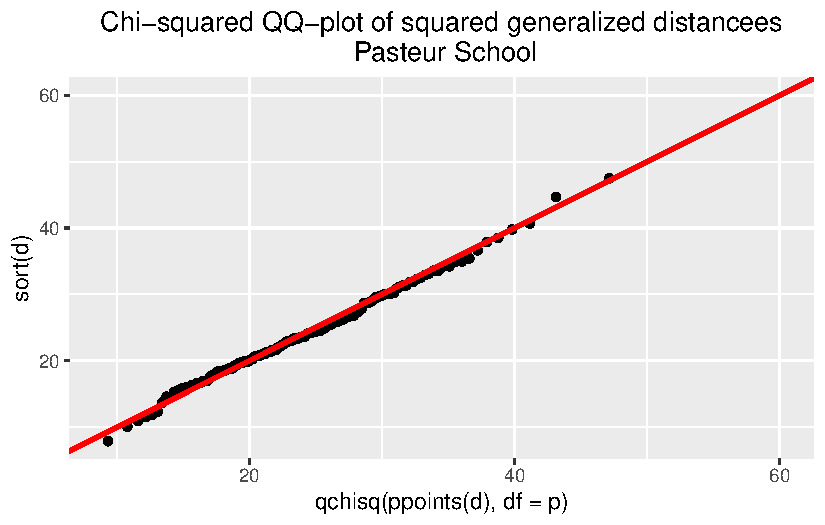
\includegraphics{ProblemSet2_files/figure-pdf/unnamed-chunk-42-1.pdf}

As we can see, the assumption of normality seems to perfectly fit the
data coming from the Pasteur school.

We can now fit the model for the Pasteur data using the
\texttt{factanal} function and 5 factors. Since we are asked to compare
the interpretation of the factors with the one obtained using data of
the students in the Grant-White school, we already perform the factor
analysis using the varimax rotation.

\begin{Shaded}
\begin{Highlighting}[]
\NormalTok{psych}\FloatTok{.5}\NormalTok{fa.ml }\OtherTok{\textless{}{-}} \FunctionTok{factanal}\NormalTok{(}\AttributeTok{x=}\NormalTok{Pasteur, }\AttributeTok{factors =}\NormalTok{ m[}\DecValTok{1}\NormalTok{], }\AttributeTok{rotation =} \StringTok{"varimax"}\NormalTok{)}
\NormalTok{psych}\FloatTok{.5}\NormalTok{fa.ml}\SpecialCharTok{$}\NormalTok{loadings}
\end{Highlighting}
\end{Shaded}

\begin{verbatim}

Loadings:
    Factor1 Factor2 Factor3 Factor4 Factor5
V1   0.314   0.578   0.138                 
V2           0.517                  -0.144 
V3           0.444  -0.177                 
V4           0.671   0.190   0.170         
V5   0.806                           0.143 
V6   0.782   0.157                   0.202 
V7   0.904                   0.109         
V8   0.684   0.169   0.139   0.152         
V9   0.775   0.249           0.102   0.156 
V10  0.141  -0.208   0.116   0.500   0.641 
V11  0.349           0.231   0.671         
V12                          0.526   0.217 
V13          0.272           0.544         
V14                  0.690                 
V15 -0.133   0.125   0.613  -0.110         
V16          0.386   0.475   0.176   0.161 
V17                  0.523   0.289         
V18  0.100           0.465                 
V19          0.244   0.357   0.241         
V20  0.123   0.514   0.189                 
V21  0.284   0.387   0.141   0.195   0.432 
V22  0.469   0.481           0.152         
V23  0.357   0.587   0.144           0.299 
V24  0.218   0.294   0.226   0.240   0.530 

               Factor1 Factor2 Factor3 Factor4 Factor5
SS loadings      3.944   2.810   2.018   1.691   1.205
Proportion Var   0.164   0.117   0.084   0.070   0.050
Cumulative Var   0.164   0.281   0.366   0.436   0.486
\end{verbatim}

Also in this case we can observe that the proportion of cumulative
variance explained by the five factors is simply equal to the 48.6\%, a
percentage that is not so satisfactory. We can also notice that the
proportion of variance explained by the last factor is doubled with
respect to the data from the Grant-White school, hence we expect a
slightly easier interpretation of the fifth factor than before.
Conversely the proportion of variance explained by factor 3 and 4 are
smaller. This may suggest the presence of some differences between the
interpretations.

We group the variable exactly as we have done for the Grant-White data:

\begin{itemize}
\tightlist
\item
  firstly, for each variable we detect its greatest loading and the
  corresponding factor;
\item
  then we assess the significance of the loading by means of a threshold
  value of 0.5.
\end{itemize}

The first group is made up by the variables:

\begin{verbatim}
  var                 meaning load.max
1  V5     general information    0.806
2  V6 paragraph comprehension    0.782
3  V7     sentence completion    0.904
4  V8     word classification    0.684
5  V9            word meaning    0.775
\end{verbatim}

All the variables in this group have high loadings, moreover the
variables in this group are exactly the same we have found in the group
related to the first common factor of the Grant-White data. Therefore we
may rightly say that, in both cases - with the Grant-White or Pasteur
data - the first common factor may be interpret as ``verbal
intelligence''.

The second group comprehends:

\begin{verbatim}
  var           meaning load.max
1  V1 visual perception    0.578
2  V2             cubes    0.517
3  V3  paper form board    0.444
4  V4             flags    0.671
5 V20         deduction    0.514
6 V22 problem reasoning    0.481
7 V23 series completion    0.587
\end{verbatim}

among which the variables with a loading higher then the fixed
significant threshold value are:

\begin{verbatim}
  var           meaning load.max
1  V1 visual perception    0.578
2  V2             cubes    0.517
3  V4             flags    0.671
4 V20         deduction    0.514
5 V23 series completion    0.587
\end{verbatim}

Even for this second group we can observe a good correspondence to what
we have found using the Grant-White data. Indeed, the variables that
load sufficiently high on this factor are almost the same then in the
previous analysis. If then we consider also the removed variables whose
loadings are smaller than 0.5, we can see a perfect correspondence
between the two groups. Hence we can still interpret this second factor
as ``visual, spatial and logic intelligence''.

Let's switch to the third group:

\begin{verbatim}
  var            meaning load.max
1 V14   word recognition    0.690
2 V15 number recognition    0.613
3 V16 figure recognition    0.475
4 V17      object-number    0.523
5 V18      number-figure    0.465
6 V19        figure-word    0.357
\end{verbatim}

and removing the variable with less significant loadings:

\begin{verbatim}
  var            meaning load.max
1 V14   word recognition    0.690
2 V15 number recognition    0.613
3 V17      object-number    0.523
\end{verbatim}

Comparing with the results obtained in the Grant-White data analysis, we
can observe that this group appears to correspond to the group which -
in that analysis - was related to the fourth factor. Despite this
inversion of order we can reasonably say that the interpretation of the
third factor we are considering and of the previous fourth factor are
basically the same. Indeed, even in this case all the identified
variables are related to the spheres of recognition.

We can also underline that the only difference among the two groups
(before ``cutting'' at 0.5) is the absence of the variable \texttt{V11}
in this latter one. This can be considered a subtle and not so relevant
disagreement: \texttt{V11} indeed had already a loading (0.436) below
the significance threshold value and actually showed other two loadings
of a very similar magnitude (0.423 in correspondence of factor 3 and
0.418 on factor 5). For all those reasons, its classification is far
more clear than in the previous analysis.

To conclude, we can assimilate this third factor to the previous fourth
one: reasonably they can be both interpreted as ``recognition skills''.

At this point we expect to see a fourth group similar to the previous
third or fifth one:

\begin{verbatim}
  var                  meaning load.max
1 V11                     code    0.671
2 V12            counting dots    0.526
3 V13 straight-curved capitals    0.544
\end{verbatim}

The result we get however is different, let's look at it. Firstly we
notice that all the variables have a loading higher then 0.5, thus all
have a level of significance that is high enough. The three variables
are at first glance not much related, nevertheless - as already
mentioned at the very beginning, during the comment relative to the
correlation plot of the Grant-White data - all these three test, in our
opinion, involve quite simple tasks for children whose age ranges
between 11 to 16 years old. For this reason, we believe that the results
of all these tests heavily rely on students ability to stay focused for
a long time and be precise, maybe even under pressure. Given this
interpretation of the test, it is quite natural to denote this factor as
``focus'' or ``precision''.

Actually, taking into account the previous difficulties in determining
the group for \texttt{V11} as well as the fact that its loading for the
fifth factor was not so small with respect to its maximum one, we may
say that the Pasteur data succeed in better identify the ``mysterious''
previous fifth factor. In other words, we believe that the last factor
of the previous analysis - that we have also pointed out as potentially
difficult to interpret due to the low proportion of variance it
explained - has instead been clearly identified using the data from the
second school.

Finally, as a further confirmation of what we have just argued, we would
like to obtain a fifth group that can be explained based on a
mathematical underlying factor. The variables classified in this last
group are:

\begin{verbatim}
  var             meaning load.max
1 V10            addition    0.641
2 V21   numerical puzzles    0.432
3 V24 arithmetic problems    0.530
\end{verbatim}

and the one with sufficiently high loadings:

\begin{verbatim}
  var             meaning load.max
1 V10            addition    0.641
2 V24 arithmetic problems    0.530
\end{verbatim}

As wished, this group suits quite well the previous third one. Therefore
the corresponding unobserved common factor can be reasonably called
``arithmetic skills''.

Before summing up what we have found, we quickly look at the variables
whose loadings are all under the significance threshold value:

\begin{verbatim}
    Factor1 Factor2 Factor3 Factor4 Factor5            meaning
V3    0.098   0.444  -0.177   0.003   0.100   paper form board
V16   0.083   0.386   0.475   0.176   0.161 figure recognition
V18   0.100  -0.005   0.465   0.089  -0.008      number-figure
V19   0.067   0.244   0.357   0.241   0.034        figure-word
V21   0.284   0.387   0.141   0.195   0.432  numerical puzzles
V22   0.469   0.481   0.029   0.152   0.051  problem reasoning
\end{verbatim}

We can see that for \texttt{V3} and \texttt{V18} the grouping appears to
reasonably holds and that also \texttt{V16} may be actually assigned to
factor 3. For what concern the last three variables things get more
complicated: \texttt{V22} loads almost equally on factor 1 and 2,
\texttt{V21} has also a not negligible loading on factor 3 and
\texttt{V19} appears to have all low loadings.

Nevertheless we may simply address this problems referring to the
transversal competences requested by the corresponding tests. The above
interpretation may still be considered quite satisfactory.

To conclude, we can say that we have found quite a good agreement
between the interpretations of the common factors based on the
Grant-White students data and on the Pasteur student data. This is
reasonable, as we expect that the underlying skills necessary to
complete the proposed attitudinal tests were the same - regardless of
the school attended by the students. Moreover, this concordance among
the results was desirable as it can be used to assess the ``stability''
of our analysis and interpretation.

\hypertarget{make-a-scatterplot-of-the-first-two-factor-scores-from-the-rotated-mlfa-solution-for-each-school.-comment.}{%
\subsubsection{5. Make a scatterplot of the first two factor scores from
the rotated MLFA solution for each school.
Comment.}\label{make-a-scatterplot-of-the-first-two-factor-scores-from-the-rotated-mlfa-solution-for-each-school.-comment.}}

Exactly as we have done for the data on the students from the
Grant-White school, we compute the factor scores related to the Pasteur
students by means of the function \texttt{factanal}, using the varimax
rotation and the regression method to compute the scores.

\begin{Shaded}
\begin{Highlighting}[]
\NormalTok{psych}\FloatTok{.5}\NormalTok{fa.ml }\OtherTok{\textless{}{-}} \FunctionTok{factanal}\NormalTok{(}\AttributeTok{x=}\NormalTok{Pasteur, }\AttributeTok{factors =}\NormalTok{ m[}\DecValTok{1}\NormalTok{], }\AttributeTok{rotation =} \StringTok{"varimax"}\NormalTok{, }
\AttributeTok{scores =} \StringTok{"regression"}\NormalTok{)}
\NormalTok{scores\_Past }\OtherTok{\textless{}{-}}\NormalTok{ psych}\FloatTok{.5}\NormalTok{fa.ml}\SpecialCharTok{$}\NormalTok{scores}
\end{Highlighting}
\end{Shaded}

We then plot the first two scores. As already justified above we expect
to see almost no correlation within the two scores and normally
distributed data with a zero vector mean and an identity covariance
matrix. Therefore we look for contour plots with an approximately
circular shape and centered in the origin of the axes.

\begin{verbatim}
  correlation
1  0.04723562
\end{verbatim}

\begin{verbatim}
                     x_bar         y_bar
Grant-White: -6.795331e-18  3.298966e-18
Pasteur:      1.260677e-16 -9.167346e-17
\end{verbatim}

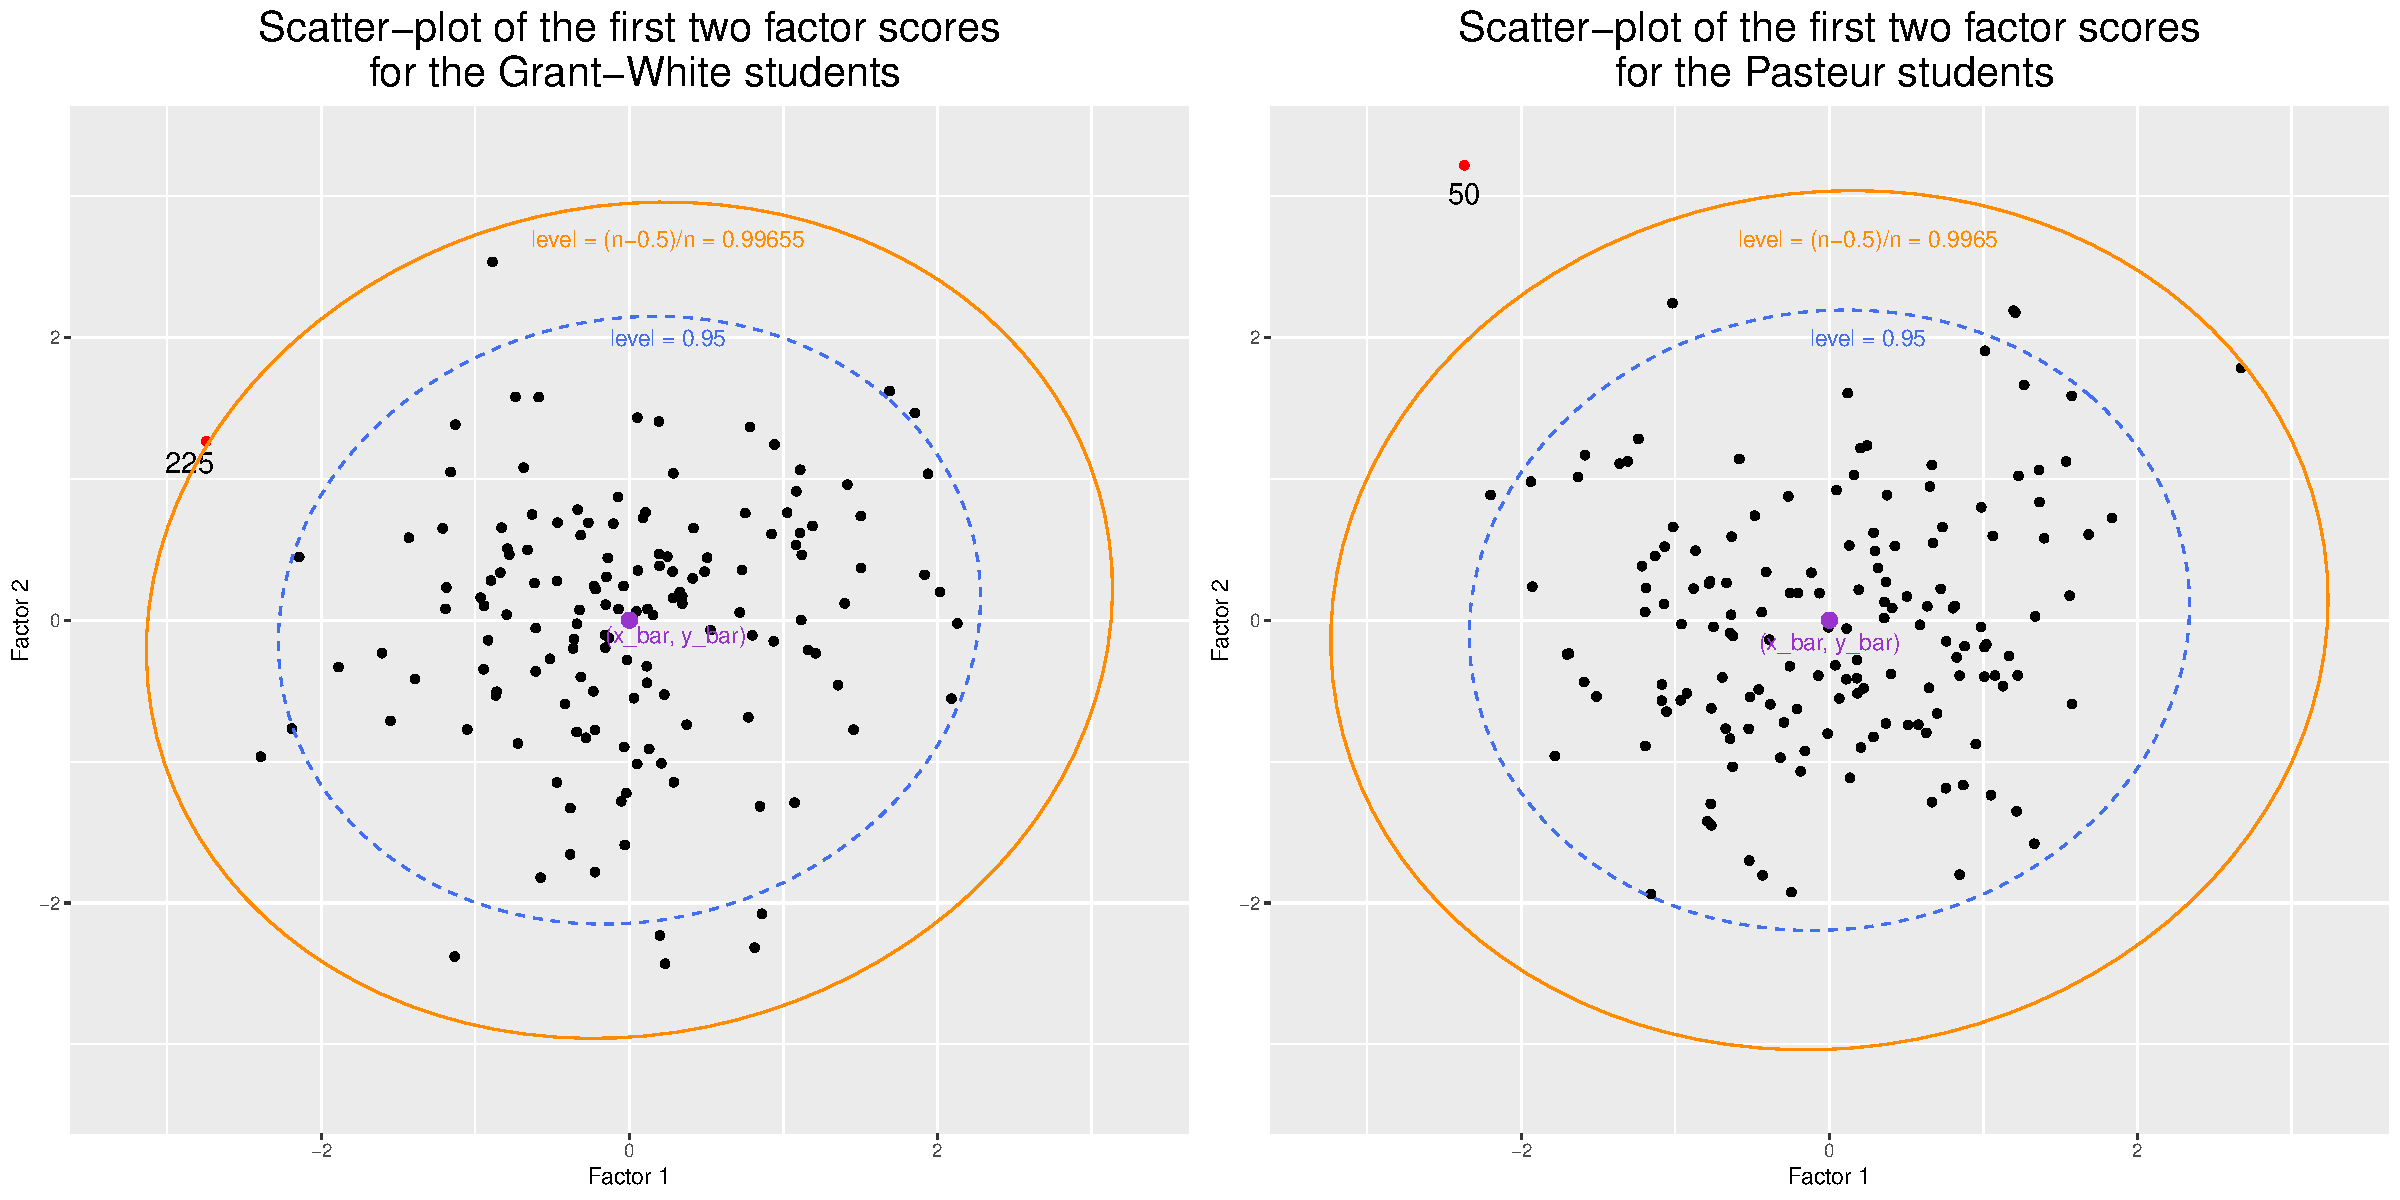
\includegraphics{ProblemSet2_files/figure-pdf/unnamed-chunk-57-1.pdf}

We again can observe that all the mentioned important features match. An
outlier is identified also in the Pasteur data, corresponding to
observations whose \texttt{Case} variable (in the original data set) has
value 50. Globally, this plot seems to agree with the Grant-White one.
Overall the two plots are very alike.

In the previous point we discussed that the first two factors for each
school have the same interpretations as ``verbal intelligence'' and
``visual, spatial and logical intelligence''. Therefore we expect the
plots to be very similar and to present the same distribution. The
similarity of the plots support even more our analysis.

\hypertarget{exercise-2}{%
\subsection{Exercise 2}\label{exercise-2}}

For exercise 2 we are going to consider the following dataset
\texttt{pendigits}:

\begin{verbatim}
   x1  y1 x2  y2  x3  y3  x4  y4 x5 y5  x6 y6  x7 y7  x8 y8 digit
1  47 100 27  81  57  37  26   0  0 23  56 53 100 90  40 98     8
2   0  89 27 100  42  75  29  45 15 15  37  0  69  2 100  6     2
3   0  57 31  68  72  90 100 100 76 75  50 51  28 25  16  0     1
4   0 100  7  92   5  68  19  45 86 34 100 45  74 23  67  0     4
5   0  67 49  83 100 100  81  80 60 60  40 40  33 20  47  0     1
6 100 100 88  99  49  74  17  47  0 16  37  0  73 16  20 20     6
\end{verbatim}

Let us start with a little data exploration in order to better
understand and interpret the results below. We note that the data-set is
missing some observations: we would expect \(44\cdot 250=11000\)
observations, but we only have \(10992\). This is almost irrelevant for
all future purposes, but we may need to be a bit more careful in the
last sections - regarding k-fold cross validation - if we want to be
accurate. We also notice that the frequencies of the digits are fairly
similar:

\begin{verbatim}

   0    1    2    3    4    5    6    7    8    9 
1143 1143 1144 1055 1144 1055 1056 1142 1055 1055 
\end{verbatim}

so we do not expect the priors to add a strong correction term in our
classifications, since they are almost uniform.

We recall that the effectiveness of linear discriminant analysis relies
on the assumption of normality of the conditional distributions of the
data given that they belong to one of the classes and the further
assumption that all these conditional distributions share the same
covariance matrix. Thus it is worth having a quick overview of how well
a Gaussian model fits the conditional distribution, and how the
covariance matrices compare with each other given different classes.

Let's start by assessing multivariate normality of the data via the
chi-square Q-Q plot of the squared Mahalanobis distances.

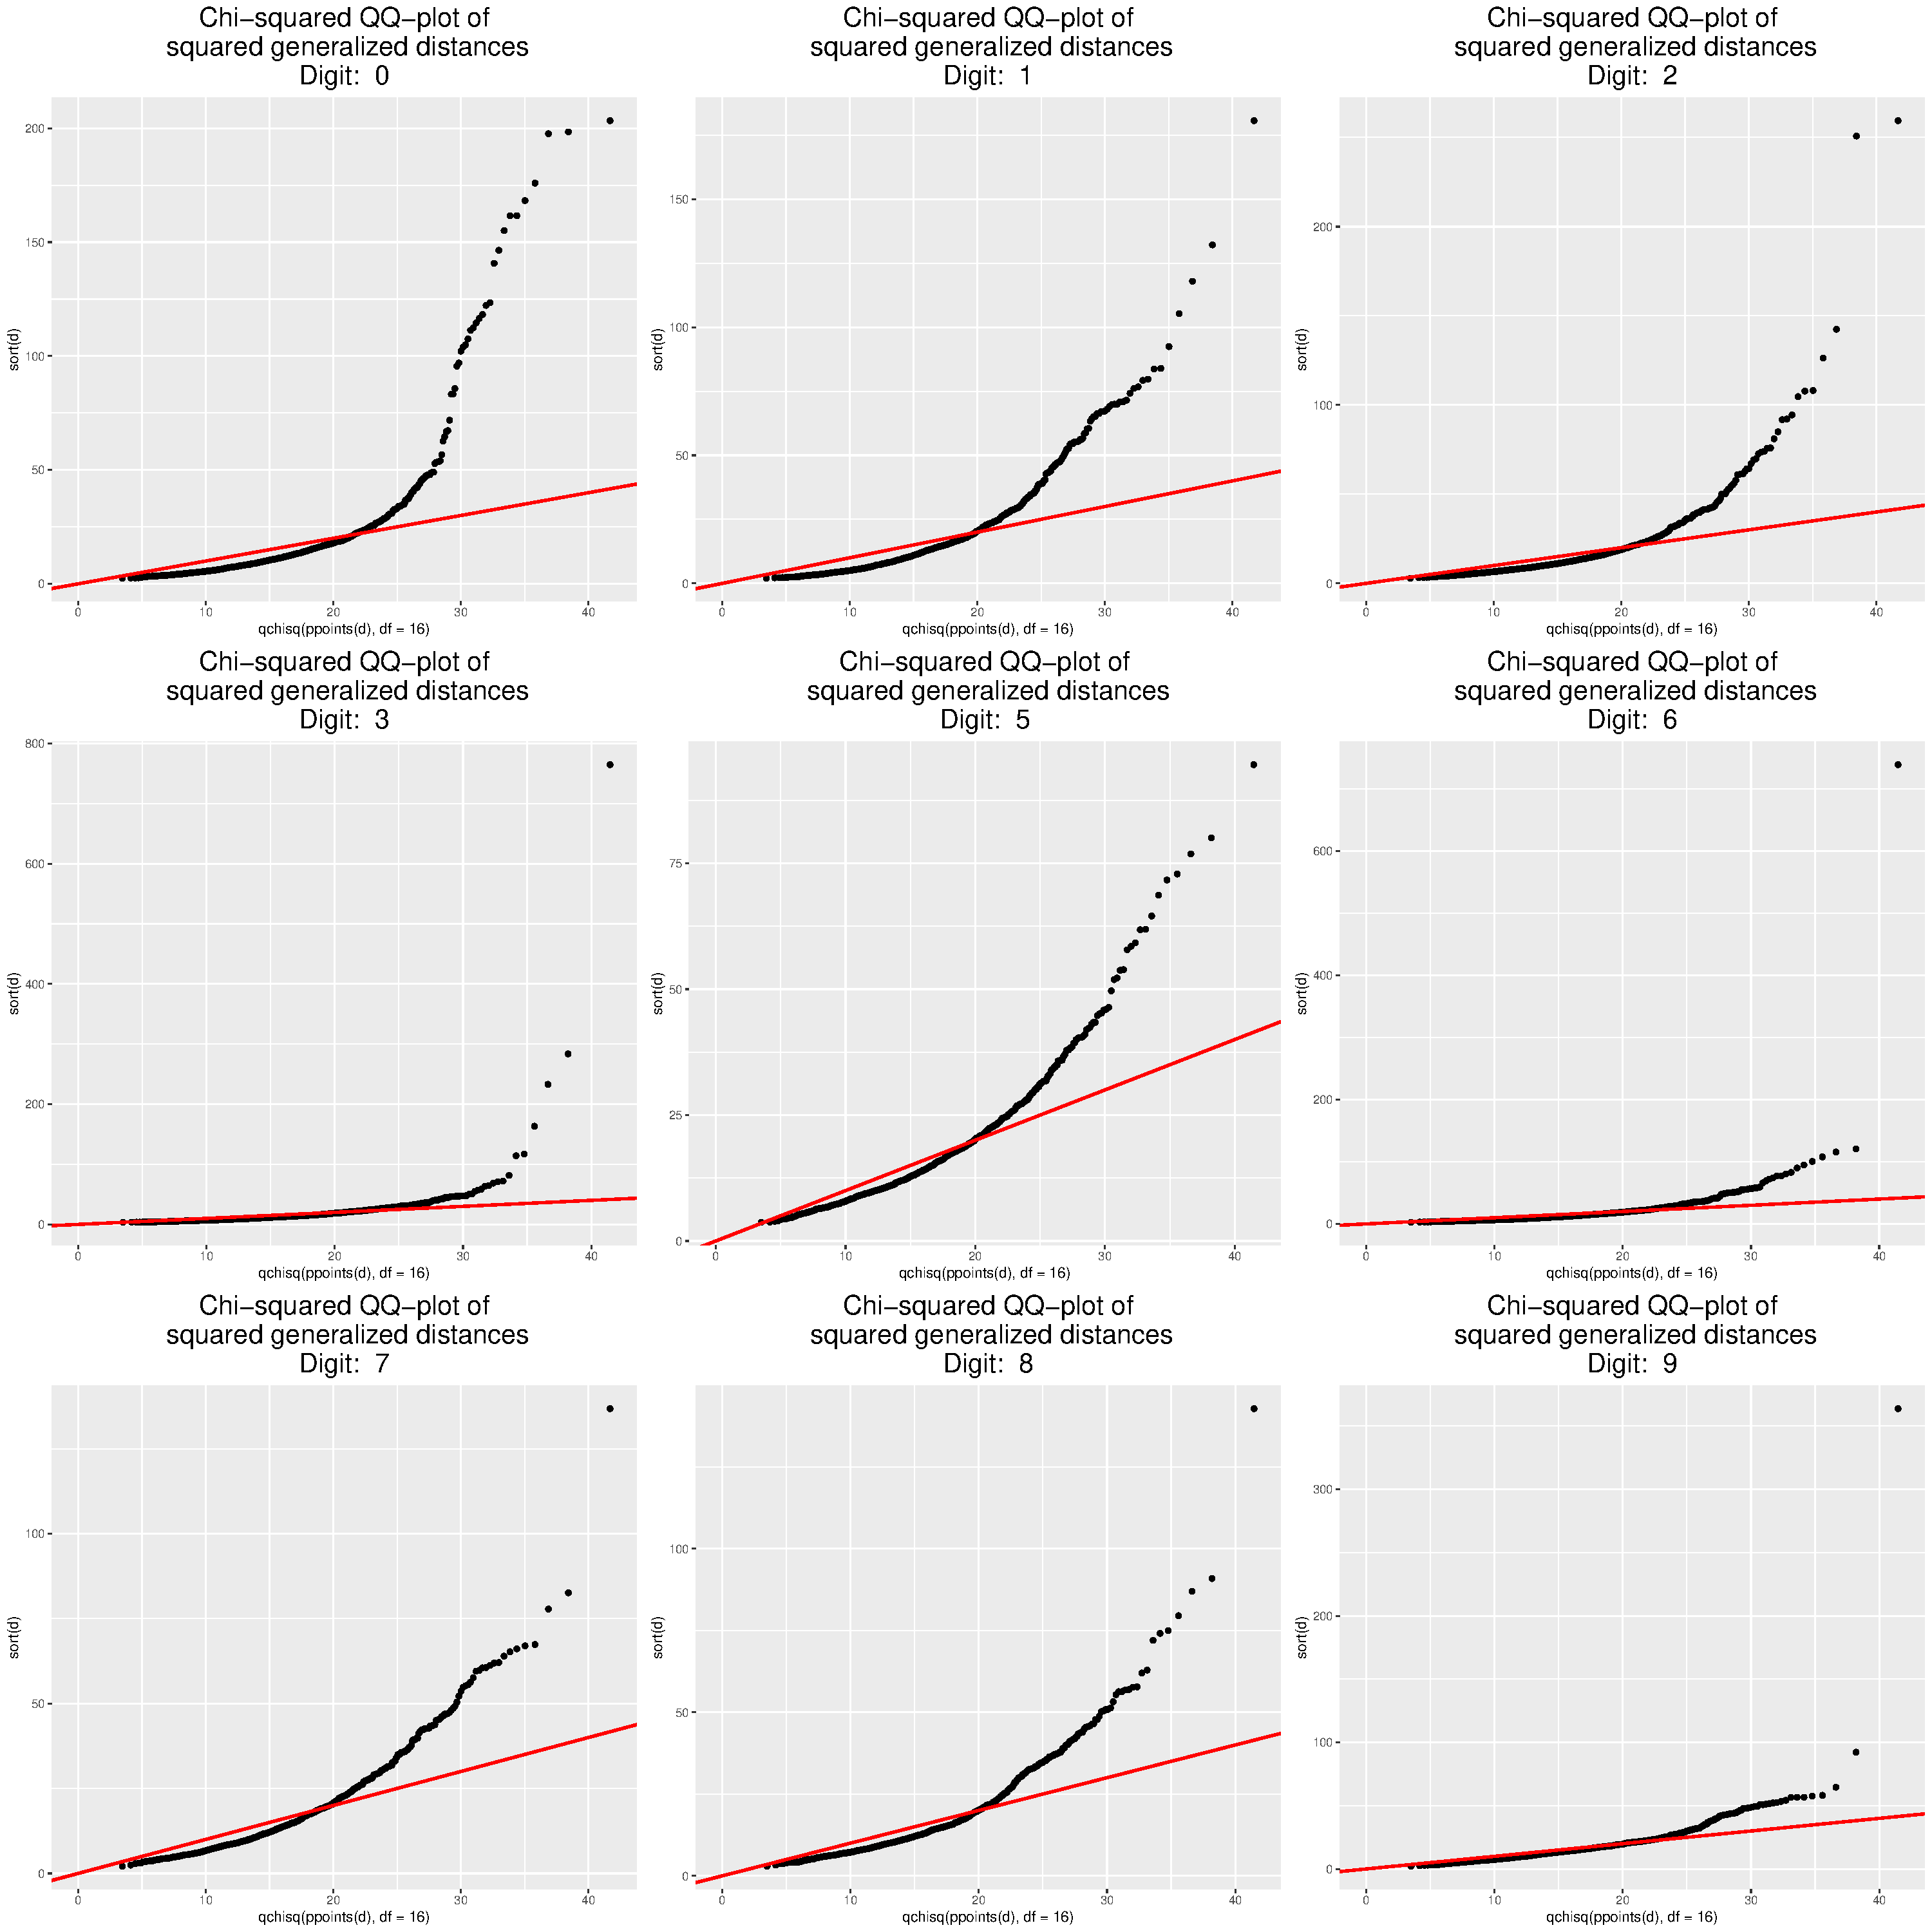
\includegraphics{ProblemSet2_files/figure-pdf/unnamed-chunk-62-1.pdf}

We left out the particular case of the digit \emph{4}, which has an
interesting feature: the variable \texttt{y8} takes value \(0\) for
every observation. This implies that it cannot be a \(16\)-dimensional
multivariate normal with ``proper dimension'' (the covariance matrix is
only positive semi-definite and the determinant is zero), but it may
still be a Gaussian vector without a pdf. To assess this, we project it
in the \(15\)-dimensional hyperplane \(\{\)\texttt{y\_8}\(=0\}\):

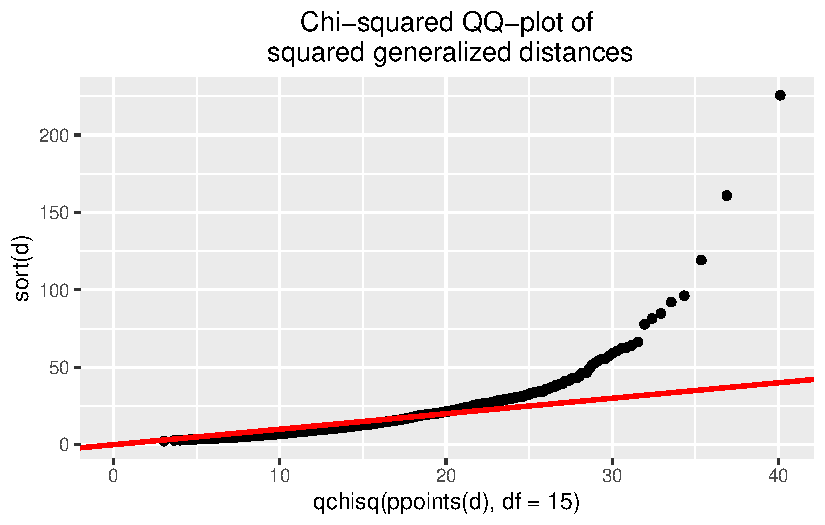
\includegraphics{ProblemSet2_files/figure-pdf/unnamed-chunk-63-1.pdf}

It seems that all these distributions suffer, to different extents, the
effects of heavier-than-expected right tails, therefore we cannot assess
gaussianity of any conditional distribution.\\
We proceed with the analysis, keeping in mind that, even if the
assumptions fail, the robustness of LDA could guarantee fairly good
results.

Now we compare variances. To check that the conditional densities all
share the same covariance matrix, we compute the Frobenius distances
between each class covariance matrix and the pooled covariance matrix,
which is ultimately the one used in LDA as estimator of the - allegedly
- shared population covariance matrix among classes.

\begin{Shaded}
\begin{Highlighting}[]
\NormalTok{covar}\OtherTok{=}\FunctionTok{list}\NormalTok{()}
\ControlFlowTok{for}\NormalTok{(i }\ControlFlowTok{in} \DecValTok{1}\SpecialCharTok{:}\DecValTok{10}\NormalTok{)\{}
\NormalTok{  by\_digit}\OtherTok{=}\NormalTok{ pendigits }\SpecialCharTok{\%\textgreater{}\%}\NormalTok{ dplyr}\SpecialCharTok{::}\FunctionTok{filter}\NormalTok{(digit}\SpecialCharTok{==}\NormalTok{(i}\DecValTok{{-}1}\NormalTok{)) }\SpecialCharTok{\%\textgreater{}\%}\NormalTok{ dplyr}\SpecialCharTok{::}\FunctionTok{select}\NormalTok{(}\SpecialCharTok{{-}}\NormalTok{digit)}
\NormalTok{  covar[i]}\OtherTok{=}\FunctionTok{list}\NormalTok{(}\FunctionTok{cov}\NormalTok{(by\_digit))}
\NormalTok{\}}

\CommentTok{\#pooled sample covariance matrix}
\NormalTok{n.k}\OtherTok{\textless{}{-}}\FunctionTok{as.numeric}\NormalTok{(}\FunctionTok{table}\NormalTok{(pendigits}\SpecialCharTok{$}\NormalTok{digit))}
\NormalTok{out}\OtherTok{\textless{}{-}}\FunctionTok{by}\NormalTok{(pendigits[,}\DecValTok{1}\SpecialCharTok{:}\DecValTok{16}\NormalTok{],pendigits}\SpecialCharTok{$}\NormalTok{digit,var)}
\NormalTok{W}\OtherTok{\textless{}{-}}\FunctionTok{matrix}\NormalTok{(}\DecValTok{0}\NormalTok{,}\AttributeTok{ncol=}\DecValTok{16}\NormalTok{,}\AttributeTok{nrow=}\DecValTok{16}\NormalTok{)}
\ControlFlowTok{for}\NormalTok{ (i }\ControlFlowTok{in} \DecValTok{1}\SpecialCharTok{:}\NormalTok{k) W}\OtherTok{\textless{}{-}}\NormalTok{W}\SpecialCharTok{+}\NormalTok{out[[i]]}\SpecialCharTok{*}\NormalTok{(n.k[i]}\SpecialCharTok{{-}}\DecValTok{1}\NormalTok{)}
\NormalTok{S}\OtherTok{\textless{}{-}}\NormalTok{W}\SpecialCharTok{/}\NormalTok{(n}\SpecialCharTok{{-}}\NormalTok{k)}

\NormalTok{f}\OtherTok{=}\FunctionTok{vector}\NormalTok{()}
\ControlFlowTok{for}\NormalTok{(i }\ControlFlowTok{in} \DecValTok{1}\SpecialCharTok{:}\DecValTok{10}\NormalTok{)\{}
\NormalTok{      f[i]}\OtherTok{=}\FunctionTok{frobenius.norm}\NormalTok{(covar[[i]]}\SpecialCharTok{{-}}\NormalTok{S)}
\NormalTok{\}}
\FunctionTok{data.frame}\NormalTok{(}\AttributeTok{digit=}\DecValTok{0}\SpecialCharTok{:}\DecValTok{9}\NormalTok{, }\AttributeTok{frobenius=}\NormalTok{f)}
\end{Highlighting}
\end{Shaded}

\begin{verbatim}
   digit frobenius
1      0  3880.912
2      1  3709.710
3      2  2166.178
4      3  2276.622
5      4  2201.819
6      5 10794.566
7      6  2318.730
8      7  2170.487
9      8  5263.531
10     9  2672.726
\end{verbatim}

We find that there are some digits, namely \emph{5}, \emph{8}, \emph{0}
and \emph{1}, for which the assumption of equal class covariance matrix
might be more ``stretched'' than for the others. We keep this in mind
for future reference, as this might be linked to worse performance of
the classification of these digits. Even more so if we consider that
also the normality assumption seemed to be unfitting, so we lack
theoretical guarantees on a good performance of LDA.

\hypertarget{use-linear-discriminant-analysis-lda.-display-the-first-two-ld-variables-in-a-scatterplot-color-coding-the-observations-according-to-variable-digit.col-below.-how-well-do-they-discriminate-the-10-digits-refer-also-to-theory.}{%
\subsubsection{1. Use linear discriminant analysis (LDA). Display the
first two LD variables in a scatterplot, color coding the observations
according to variable digit.col below. How well do they discriminate the
10 digits? Refer also to
theory.}\label{use-linear-discriminant-analysis-lda.-display-the-first-two-ld-variables-in-a-scatterplot-color-coding-the-observations-according-to-variable-digit.col-below.-how-well-do-they-discriminate-the-10-digits-refer-also-to-theory.}}

First of all, as requested, we proceed by implementing the linear
discriminant analysis:

\begin{Shaded}
\begin{Highlighting}[]
\NormalTok{lda.fit }\OtherTok{\textless{}{-}}\NormalTok{ MASS}\SpecialCharTok{::}\FunctionTok{lda}\NormalTok{(digit }\SpecialCharTok{\textasciitilde{}}\NormalTok{ ., }\AttributeTok{data =}\NormalTok{ pendigits)}
\NormalTok{lda.fit}
\end{Highlighting}
\end{Shaded}

\begin{verbatim}
Call:
lda(digit ~ ., data = pendigits)

Prior probabilities of groups:
         0          1          2          3          4          5          6 
0.10398472 0.10398472 0.10407569 0.09597889 0.10407569 0.09597889 0.09606987 
         7          8          9 
0.10389374 0.09597889 0.09597889 

Group means:
         x1       y1       x2       y2        x3       y3        x4        y4
0 35.372703 86.06387 11.57743 58.31059 14.935258 19.60017 51.172353  7.293963
1 14.702537 61.39283 44.35171 77.93526 69.857393 89.50919 77.496938 79.800525
2 18.392483 76.94930 42.13024 99.38724 67.460664 79.76136 51.276224 46.046329
3 24.784834 84.06066 56.65972 99.51943 86.644550 84.68720 64.525118 60.589573
4 42.958042 99.54021 22.12587 79.37850  5.752622 51.15822 42.833916 40.470280
5 41.239810 90.94313 42.59810 75.83128 57.313744 59.17915 36.459716 29.355450
6 87.520833 98.71970 51.75379 86.72443 20.709280 58.48295  6.942235 26.928030
7  3.497373 91.00876 45.37128 98.24869 78.846760 80.75832 71.266200 47.467601
8 56.948815 82.08057 39.83033 79.61517 51.814218 51.92796 50.564929 24.221801
9 69.263507 81.31848 52.79336 83.25972 45.450237 81.27867 56.568720 82.956398
        x5        y5       x6        y6       x7        y7        x8        y8
0 85.94138 31.301837 89.29484 68.492563 59.01137 89.312336 22.096238 75.237970
1 67.63780 54.059493 47.80140 32.657918 44.60105 16.157480 59.905512  1.382327
2 19.83129 19.378497 11.63986  9.093531 53.05769  5.246503 98.710664  4.171329
3 82.12891 43.217062 90.88246 17.257820 50.01327  2.275829  3.468246  6.244550
4 85.10315 49.561189 86.29895 59.722902 70.98951 31.452797 62.603147  0.000000
5 26.18389 33.152607 37.63602 50.236019 42.83128 57.687204 59.459716 60.308057
6 32.60511  3.143939 81.10890 11.018939 61.57197 30.538826 11.000000 23.353220
7 52.72942 14.933450 33.60333 18.471103 39.51138 33.798599 81.143608 34.306480
8 35.24834 17.066351 39.92607 36.896682 67.78483 68.488152 48.997156 81.403791
9 79.05972 71.091943 89.78009 43.232227 61.47867 14.340284 18.151659  4.536493

Coefficients of linear discriminants:
            LD1          LD2          LD3           LD4          LD5
x1  0.017031469  0.010842533  0.001099055 -0.0301920463 -0.009628500
y1  0.010496495  0.030217727 -0.018628117  0.0291497539 -0.008436276
x2  0.006154561 -0.002398809 -0.002384957  0.0115389533 -0.016430580
y2 -0.034121100 -0.038556558 -0.011397075  0.0127154842  0.042296258
x3 -0.024329618 -0.022268517 -0.012254083 -0.0172261636  0.025711725
y3  0.003846840  0.004680081 -0.018446935 -0.0137205754 -0.035142025
x4 -0.006772741  0.005488090  0.005636164  0.0070198022 -0.013664106
y4  0.015380360 -0.012348136  0.010162746 -0.0004200916  0.007220528
x5  0.002884508 -0.008763204 -0.024379942  0.0111882478  0.033003482
y5 -0.011847742 -0.009512370 -0.031145068 -0.0133473343 -0.021389031
x6  0.011499150  0.019019773 -0.006394341 -0.0101616113  0.007274599
y6 -0.001588012  0.015872651 -0.062483853 -0.0081810793 -0.020143865
x7 -0.002137111 -0.006247144  0.007383929 -0.0002032483  0.004538669
y7  0.023485579 -0.008138420  0.057074710  0.0382822350  0.012546513
x8 -0.020739921  0.017834059 -0.015692938  0.0087462786 -0.013853138
y8  0.032188123 -0.052611219 -0.052393868 -0.0208986103 -0.014225393
            LD6          LD7          LD8           LD9
x1 -0.005225432  0.010988539 -0.010242776 -0.0007957003
y1 -0.043106769 -0.050848880 -0.026184593  0.0195143059
x2  0.009815750 -0.026965684 -0.005197915  0.0113807824
y2 -0.010020819  0.037222629 -0.050101644 -0.0699867378
x3 -0.019124373  0.017963095 -0.009816410  0.0010125072
y3 -0.018566351 -0.033394354  0.045196577  0.0950500001
x4  0.013338321 -0.011818355  0.001495475  0.0050668206
y4  0.050875676 -0.044286619 -0.062853651 -0.0584064518
x5  0.015518994  0.015504881 -0.016579084  0.0249044629
y5 -0.028889344  0.029151571  0.024961776 -0.0283297770
x6 -0.020431468 -0.027084489  0.015244884 -0.0311859130
y6 -0.030850311  0.009254166 -0.006245133  0.0384201568
x7  0.028312603  0.036613456 -0.035868084  0.0438862999
y7  0.062898041 -0.049573456 -0.017105111 -0.0183390804
x8 -0.010046723 -0.008412180 -0.004655399 -0.0187797367
y8 -0.033519031  0.012519110 -0.003984131 -0.0072610469

Proportion of trace:
   LD1    LD2    LD3    LD4    LD5    LD6    LD7    LD8    LD9 
0.4246 0.1877 0.1206 0.0851 0.0725 0.0502 0.0365 0.0197 0.0031 
\end{verbatim}

Note that, by default, the priors are the proportions of occurrences of
each class in the data set, and they are all pretty similar.

\begin{Shaded}
\begin{Highlighting}[]
\NormalTok{lda.pred }\OtherTok{\textless{}{-}} \FunctionTok{predict}\NormalTok{(lda.fit)}
\end{Highlighting}
\end{Shaded}

We can now display the first two LD variables in the below scatterplot,
which gives the ``optimal'' bi-dimensional representation of the data
for ``separation purposes'' (i.e.~with minimized within-class variance
and maximized between-class variance). Note that the assumptions under
which this optimality holds, as previously discussed, are not really
met, but we still expect a good result:

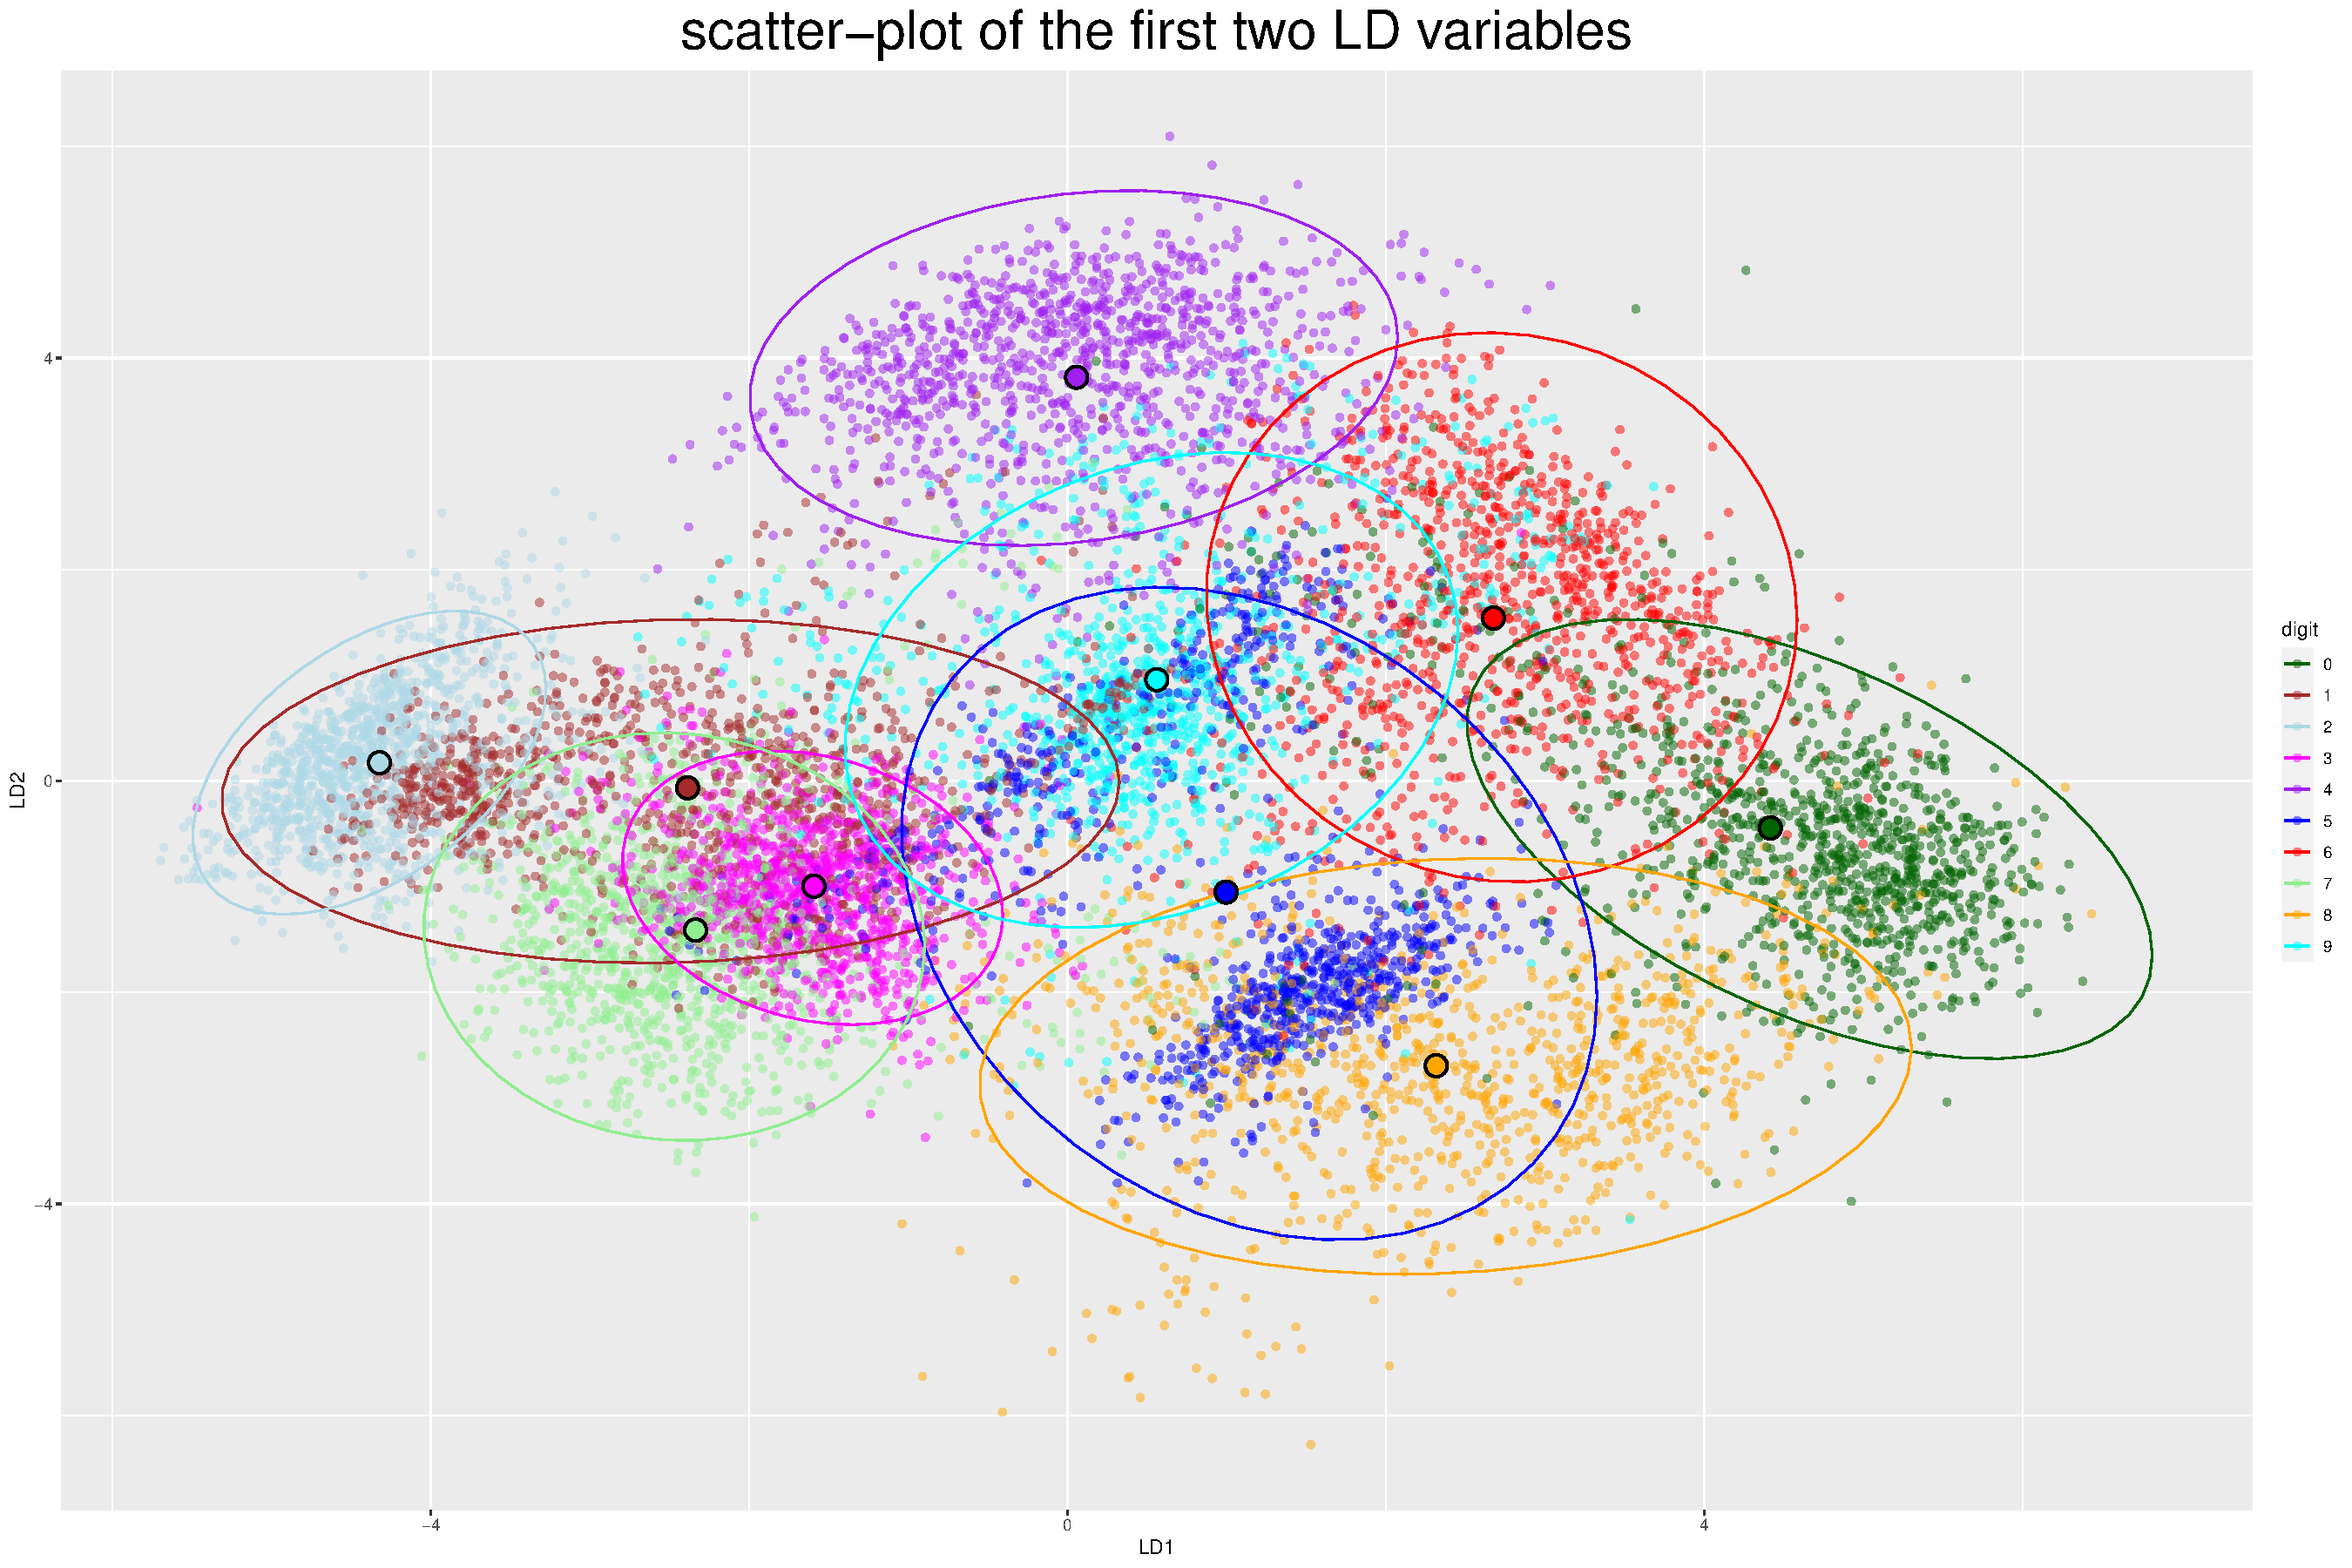
\includegraphics{ProblemSet2_files/figure-pdf/unnamed-chunk-68-1.pdf}

An analysis of the considered scatterplot should therefore give an idea
of the overall behavior of the classifier. However, since the proportion
of trace of the first two LDs is just around \(0.6\), we do not expect
the information provided by the plot to be entirely accurate for a full
rank LDA.\\
In the plot we can appreciate that the digit \emph{4} forms a clear and
compact cloud at the top, and so does \emph{2} at the left. Meanwhile
the other digits have clouds with some values far away from the
centroids (the points highlighted by the black boundaries). The worst
case seems to be digit \emph{5}, which appears to have somewhat of a
``bi-modal projected distribution'', with points concentrated in two
separated regions. Digits \emph{0} and \emph{8} show some overlap with
the neighboring ones, and \emph{1} even more than them. In general all
the other digits do not form a compact distribution around their
centroids and display very different variances in the LD1-LD2 plane.

We can also observe that the first two discriminant directions do a
quite good job in separating the class centroids, as their associated
coordinates on the respective axes are all quite different from one
another. In particular, LD1 seems to ``isolate'' quite well the
centroids associated to \emph{0} and \emph{2}, whereas LD2 does the same
for \emph{4} and \emph{8}. Conversely, \emph{1}, \emph{3} and \emph{7}
appear to be all ``clustered together'' by the first two LDs.

We can start making some speculations, that we will investigate better
in the analysis below.\\
Digit \emph{5} could be confused with \emph{9} due to their considerable
overlapping area: we could have suspected it, considering how similar
their shapes are. The same goes for \emph{8} and \emph{0}.\\
This outcome could arise from the fact that the assumptions under which
the optimal discrimination holds, as previously shown, are not fully
met, as well as the fact that the proportion of trace explained by the
first two LDs is not satisfactory.

\hypertarget{compute-the-confusion-matrix-on-the-training-data.-what-are-the-groups-more-difficult-to-discriminate-from-the-others-comment-in-view-of-the-answer-to-point-1.}{%
\subsubsection{2. Compute the confusion matrix on the training data.
What are the groups more difficult to discriminate from the others?
Comment in view of the answer to point
1.}\label{compute-the-confusion-matrix-on-the-training-data.-what-are-the-groups-more-difficult-to-discriminate-from-the-others-comment-in-view-of-the-answer-to-point-1.}}

In order to have a better understanding of how well the first two LD
variables discriminate the ten digits, we compute the confusion matrix
on the training data:

\begin{Shaded}
\begin{Highlighting}[]
\NormalTok{conf.mat }\OtherTok{\textless{}{-}} \FunctionTok{table}\NormalTok{(}\AttributeTok{predicted=}\NormalTok{lda.pred}\SpecialCharTok{$}\NormalTok{class,}\AttributeTok{true=}\NormalTok{pendigits}\SpecialCharTok{$}\NormalTok{digit)}
\NormalTok{conf.mat }\OtherTok{\textless{}{-}} \FunctionTok{addmargins}\NormalTok{(conf.mat)}
\NormalTok{conf.mat}
\end{Highlighting}
\end{Shaded}

\begin{verbatim}
         true
predicted     0     1     2     3     4     5     6     7     8     9   Sum
      0    1015     0     0     0     0     0     4     1    76     1  1097
      1      10   799    23    19     0     3     0    61    18    64   997
      2       0   206  1113     1     1     0     0    16     0     0  1337
      3       0    16     1  1020     1    58     0    19    10    10  1135
      4      33     2     0     0  1116     0     3     7     0    20  1181
      5       0    51     0     0     0   714     5     5    57    12   844
      6       5     7     0     0     4     3  1029     0     6     1  1055
      7       0    29     7    13     1     0     0  1015     2     0  1067
      8      77     0     0     0     0     9    15     6   875     2   984
      9       3    33     0     2    21   268     0    12    11   945  1295
      Sum  1143  1143  1144  1055  1144  1055  1056  1142  1055  1055 10992
\end{verbatim}

We also print the misclassifications for each digit:

\begin{verbatim}
  misclassifications misclassification.rates
0                128                   0.112
1                344                   0.301
2                 31                   0.027
3                 35                   0.033
4                 28                   0.024
5                341                   0.323
6                 27                   0.026
7                127                   0.111
8                180                   0.171
9                110                   0.104
\end{verbatim}

\begin{verbatim}
Using digit as id variables
\end{verbatim}

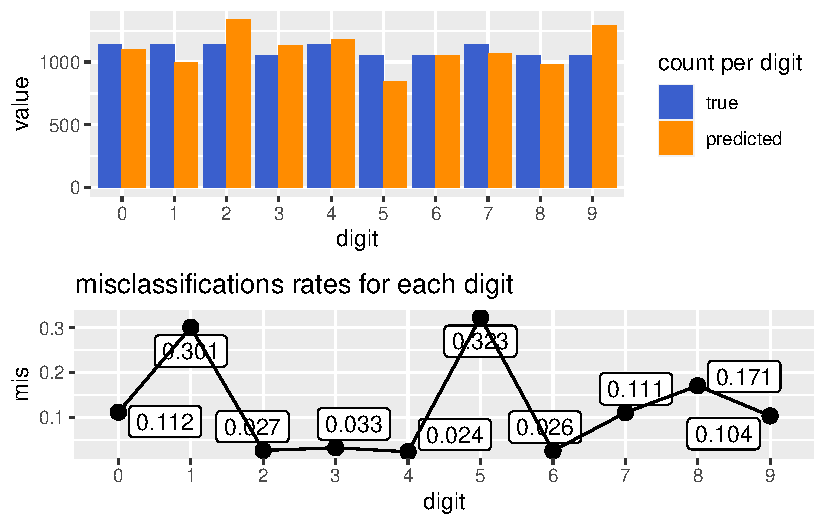
\includegraphics{ProblemSet2_files/figure-pdf/unnamed-chunk-71-1.pdf}

In the confusion matrix we can see similar patterns to the scatterplot:
the digit \emph{4} is well discriminated, it has only 28
misclassifications out of 1144 occurrences. It is interesting to note
that, as previously speculated, the digit \emph{5} has been wrongly
predicted as \emph{9} 268 times and the digit \emph{0} as \emph{8} 77
times. We also remark that the digit \emph{5} has the highest
misclassification rate, as suggested by the scatterplot. Another
interesting feature that arises from the confusion matrix is how some
digits are misclassified predominantly in one direction. For example the
digit \emph{1} has been misclassified as \emph{2} \(206\) times,
meanwhile the digit \emph{2} as \emph{1} only \(23\) times. This was
already suggested by the scatterplot: due to the high variance of the
digit \emph{1} a lot of its observations are close to the centroid of
the digit \emph{2} and so they may end up being classified as \(2\) by
the nearest centroid classification. This clearly does not apply in the
opposite direction.\\
Finally, note that the digits that are misclassified more often are also
those that we found to have a class covariance matrix ``more distant''
from the pooled one compared to those with better misclassification
rates.

\hypertarget{use-the-leave-one-out-cross-validation-cv.-compute-the-confusion-matrix-and-the-corresponding-cv-errors.-is-it-larger-than-the-training-error-why-so}{%
\subsubsection{3. Use the leave-one-out cross validation (CV). Compute
the confusion matrix and the corresponding CV errors. Is it larger than
the training error? Why
so?}\label{use-the-leave-one-out-cross-validation-cv.-compute-the-confusion-matrix-and-the-corresponding-cv-errors.-is-it-larger-than-the-training-error-why-so}}

As requested, we proceed with the leave-one-out cross validations:

\begin{Shaded}
\begin{Highlighting}[]
\NormalTok{lda.fitCV}\OtherTok{\textless{}{-}}\FunctionTok{lda}\NormalTok{(digit}\SpecialCharTok{\textasciitilde{}}\NormalTok{.,}\AttributeTok{data=}\NormalTok{pendigits, }\AttributeTok{CV=}\ConstantTok{TRUE}\NormalTok{)}
\end{Highlighting}
\end{Shaded}

And we compute the corresponding confusion matrix.

\begin{Shaded}
\begin{Highlighting}[]
\NormalTok{conf.mat}\OtherTok{\textless{}{-}}\FunctionTok{table}\NormalTok{(}\AttributeTok{predicted=}\NormalTok{lda.fitCV}\SpecialCharTok{$}\NormalTok{class,}\AttributeTok{true=}\NormalTok{pendigits}\SpecialCharTok{$}\NormalTok{digit)}
\FunctionTok{addmargins}\NormalTok{(conf.mat)}
\end{Highlighting}
\end{Shaded}

\begin{verbatim}
         true
predicted     0     1     2     3     4     5     6     7     8     9   Sum
      0    1013     0     0     0     0     0     4     1    79     1  1098
      1      10   798    23    19     1     3     0    61    18    65   998
      2       0   206  1113     1     2     0     0    17     0     0  1339
      3       0    16     1  1020     1    58     0    20    10    10  1136
      4      34     2     0     0  1115     0     3     7     0    20  1181
      5       0    51     0     0     0   712     5     5    57    13   843
      6       5     8     0     0     4     3  1029     0     7     1  1057
      7       0    29     7    13     1     0     0  1013     2     0  1065
      8      78     0     0     0     0     9    15     6   871     2   981
      9       3    33     0     2    20   270     0    12    11   943  1294
      Sum  1143  1143  1144  1055  1144  1055  1056  1142  1055  1055 10992
\end{verbatim}

We compare the training error of LDA without CV, with the one achieved
via leave-one-out cross validation:

\begin{Shaded}
\begin{Highlighting}[]
\NormalTok{training.err}\OtherTok{\textless{}{-}}\DecValTok{1}\SpecialCharTok{{-}}\FunctionTok{mean}\NormalTok{(lda.pred}\SpecialCharTok{$}\NormalTok{class}\SpecialCharTok{==}\NormalTok{pendigits}\SpecialCharTok{$}\NormalTok{digit)}
\NormalTok{CV.err}\OtherTok{\textless{}{-}}\DecValTok{1}\SpecialCharTok{{-}}\FunctionTok{mean}\NormalTok{(lda.fitCV}\SpecialCharTok{$}\NormalTok{class}\SpecialCharTok{==}\NormalTok{pendigits}\SpecialCharTok{$}\NormalTok{digit)}
\FunctionTok{data.frame}\NormalTok{(}\StringTok{"training error"}\OtherTok{=}\NormalTok{training.err, }\StringTok{"CV error"} \OtherTok{=}\NormalTok{ CV.err)}
\end{Highlighting}
\end{Shaded}

\begin{verbatim}
  training.error  CV.error
1      0.1229076 0.1241812
\end{verbatim}

As we can see, the test error rate achieved via leave-one-out cross
validation turns out to be bigger than the training error. This is to be
expected: the training error is a very over-confident estimate of the
Actual Error Rates, because it tests its performance on the same data
used to train it (so it suffers a form of ``overfitting'' to the data).
The leave-one-out CV procedure instead tests models, trained on all data
minus a single observation, on that observation and averages the error
rates obtained by repeating this procedure on each observation. It is a
more realistic measure of how well the model would fare with unseen data
(and thus tends to give a less-optimistic approximation of the AER).\\
Still, the difference of the rates is not very appreciable. This might
have to do with the fact that leaving a single handwritten digit out has
only a marginal impact on the predictive capability of that digit as the
model is trained on (around) 249 other digits from the same writer -
plus the ones of all other 33 authors.

\hypertarget{compute-the-44-fold-cross-validation-error-for-each-reduced-rank-lda-classifier-including-full-rank-lda-by-using-the-partition-of-the-observation-provided-by-the-variable-groupcv-below.-plot-the-error-curve-against-the-number-of-discriminant-variables.-what-classifier-do-you-prefer-comment.}{%
\subsubsection{\texorpdfstring{4. Compute the \(44\)-fold cross
validation error for each reduced-rank LDA classifier, including
full-rank LDA, by using the partition of the observation provided by the
variable \texttt{groupCV} below. Plot the error curve against the number
of discriminant variables. What classifier do you prefer?
Comment.}{4. Compute the 44-fold cross validation error for each reduced-rank LDA classifier, including full-rank LDA, by using the partition of the observation provided by the variable groupCV below. Plot the error curve against the number of discriminant variables. What classifier do you prefer? Comment.}}\label{compute-the-44-fold-cross-validation-error-for-each-reduced-rank-lda-classifier-including-full-rank-lda-by-using-the-partition-of-the-observation-provided-by-the-variable-groupcv-below.-plot-the-error-curve-against-the-number-of-discriminant-variables.-what-classifier-do-you-prefer-comment.}}

Let's start by observing that \(44\) is also the number of different
writers who contributed to writing the digits for the training data. If
we were under the assumption that the observations were grouped in order
of their ``author'', this \(44\)-fold cross validation could turn out to
be a very effective way of measuring the predictive capability of our
model: we would effectively test how well observation from an ``unseen''
(as in: left out from the training) writer are classified based on the
training data of the remaining \(43\). However, given the information
available on the data-set, we cannot be sure that this is the case.\\
In the following section we will use two different \(44\)-fold cross
validation error estimates: one that takes a simple average of the error
rates over all folds, and one that takes an average of those
fold-related error rates weighted on the amount of test data of said
folds, to account for the fact that the last group of test data is
slightly smaller than the others. The latter is, in essence, the total
misclassification rate of the model: it simply amounts to dividing the
total number of misclassifications over all the folds and dividing it by
the size of the dataset. Since the difference in size of the last fold
is of only \(8\) observations out of \(250\) we do not expect a sensible
difference.

\begin{Shaded}
\begin{Highlighting}[]
\NormalTok{k\_f}\OtherTok{=}\DecValTok{44}

\CommentTok{\# Initialize error rates vector}
\NormalTok{err}\OtherTok{=}\FunctionTok{matrix}\NormalTok{( }\AttributeTok{nrow=}\NormalTok{k\_f, }\AttributeTok{ncol=}\FunctionTok{min}\NormalTok{(k}\DecValTok{{-}1}\NormalTok{,p) )}
\NormalTok{mis}\OtherTok{=}\FunctionTok{rep}\NormalTok{(}\DecValTok{0}\NormalTok{, }\FunctionTok{min}\NormalTok{(k}\DecValTok{{-}1}\NormalTok{, p))}
\NormalTok{train\_err }\OtherTok{=} \FunctionTok{rep}\NormalTok{(}\DecValTok{0}\NormalTok{, }\FunctionTok{min}\NormalTok{(k}\DecValTok{{-}1}\NormalTok{, p))}

\CommentTok{\#Loop over folds}
\ControlFlowTok{for}\NormalTok{ (i }\ControlFlowTok{in} \DecValTok{1}\SpecialCharTok{:}\NormalTok{k\_f) \{}
  \CommentTok{\# Define test and train sets}
\NormalTok{  test}\OtherTok{=}\NormalTok{(groupCV }\SpecialCharTok{==}\NormalTok{ i)}
\NormalTok{  train}\OtherTok{=}\SpecialCharTok{!}\NormalTok{test}
  
  \CommentTok{\# Fit LDA model on training data}
\NormalTok{  lda.fit }\OtherTok{=} \FunctionTok{lda}\NormalTok{(digit}\SpecialCharTok{\textasciitilde{}}\NormalTok{.,}\AttributeTok{data=}\NormalTok{pendigits[train,])}
  
  \ControlFlowTok{for}\NormalTok{(j }\ControlFlowTok{in} \DecValTok{1}\SpecialCharTok{:}\FunctionTok{min}\NormalTok{(k}\DecValTok{{-}1}\NormalTok{,p))\{}
    \CommentTok{\# Predict test data using LDA model}
\NormalTok{    lda.pred }\OtherTok{=} \FunctionTok{predict}\NormalTok{(lda.fit, pendigits[test,], }\AttributeTok{dimen =}\NormalTok{ j)}\SpecialCharTok{$}\NormalTok{class}
\NormalTok{    lda.pred\_train }\OtherTok{=} \FunctionTok{predict}\NormalTok{(lda.fit, pendigits[train,], }\AttributeTok{dimen =}\NormalTok{ j)}\SpecialCharTok{$}\NormalTok{class}
    
    \CommentTok{\# Compute error rates}
\NormalTok{    train\_err[j] }\OtherTok{=}\NormalTok{ train\_err[j]}\SpecialCharTok{+}\FunctionTok{sum}\NormalTok{(lda.pred\_train }\SpecialCharTok{!=}\NormalTok{ pendigits}\SpecialCharTok{$}\NormalTok{digit[train])}
\NormalTok{    mis[j] }\OtherTok{=}\NormalTok{ mis[j]}\SpecialCharTok{+}\FunctionTok{sum}\NormalTok{(lda.pred }\SpecialCharTok{!=}\NormalTok{ pendigits}\SpecialCharTok{$}\NormalTok{digit[test])}
\NormalTok{    err[i,j] }\OtherTok{=} \DecValTok{1} \SpecialCharTok{{-}} \FunctionTok{sum}\NormalTok{(lda.pred }\SpecialCharTok{==}\NormalTok{ pendigits}\SpecialCharTok{$}\NormalTok{digit[test])}\SpecialCharTok{/}\FunctionTok{length}\NormalTok{(lda.pred)}
\NormalTok{  \}}
\NormalTok{\}}
\NormalTok{error44}\OtherTok{=}\FunctionTok{colMeans}\NormalTok{(err)}
\NormalTok{mis\_rate44}\OtherTok{=}\NormalTok{mis}\SpecialCharTok{/}\NormalTok{n}
\NormalTok{train\_err44 }\OtherTok{=}\NormalTok{ train\_err}\SpecialCharTok{/}\NormalTok{((k\_f }\SpecialCharTok{{-}}\DecValTok{1}\NormalTok{)}\SpecialCharTok{*}\NormalTok{n)}

\FunctionTok{data.frame}\NormalTok{(}\StringTok{"rank"}\OtherTok{=}\DecValTok{1}\SpecialCharTok{:}\DecValTok{9}\NormalTok{, }\StringTok{"training errors"} \OtherTok{=}\NormalTok{ train\_err44, }
       \StringTok{"arithmetic mean of errors"}\OtherTok{=}\NormalTok{error44,}
\StringTok{"misclassification rate"}\OtherTok{=}\NormalTok{mis\_rate44)}
\end{Highlighting}
\end{Shaded}

\begin{verbatim}
  rank training.errors arithmetic.mean.of.errors misclassification.rate
1    1       0.5439410                 0.5491300              0.5491266
2    2       0.3234953                 0.3244313              0.3244178
3    3       0.2513689                 0.2530075              0.2530022
4    4       0.2138342                 0.2145289              0.2145197
5    5       0.1637406                 0.1652261              0.1652111
6    6       0.1399517                 0.1416476              0.1416485
7    7       0.1329677                 0.1347355              0.1347344
8    8       0.1245324                 0.1259144              0.1259098
9    9       0.1229118                 0.1242810              0.1242722
\end{verbatim}

As expected, the differences are hardly noticeable.

\begin{verbatim}
Using rank as id variables
\end{verbatim}

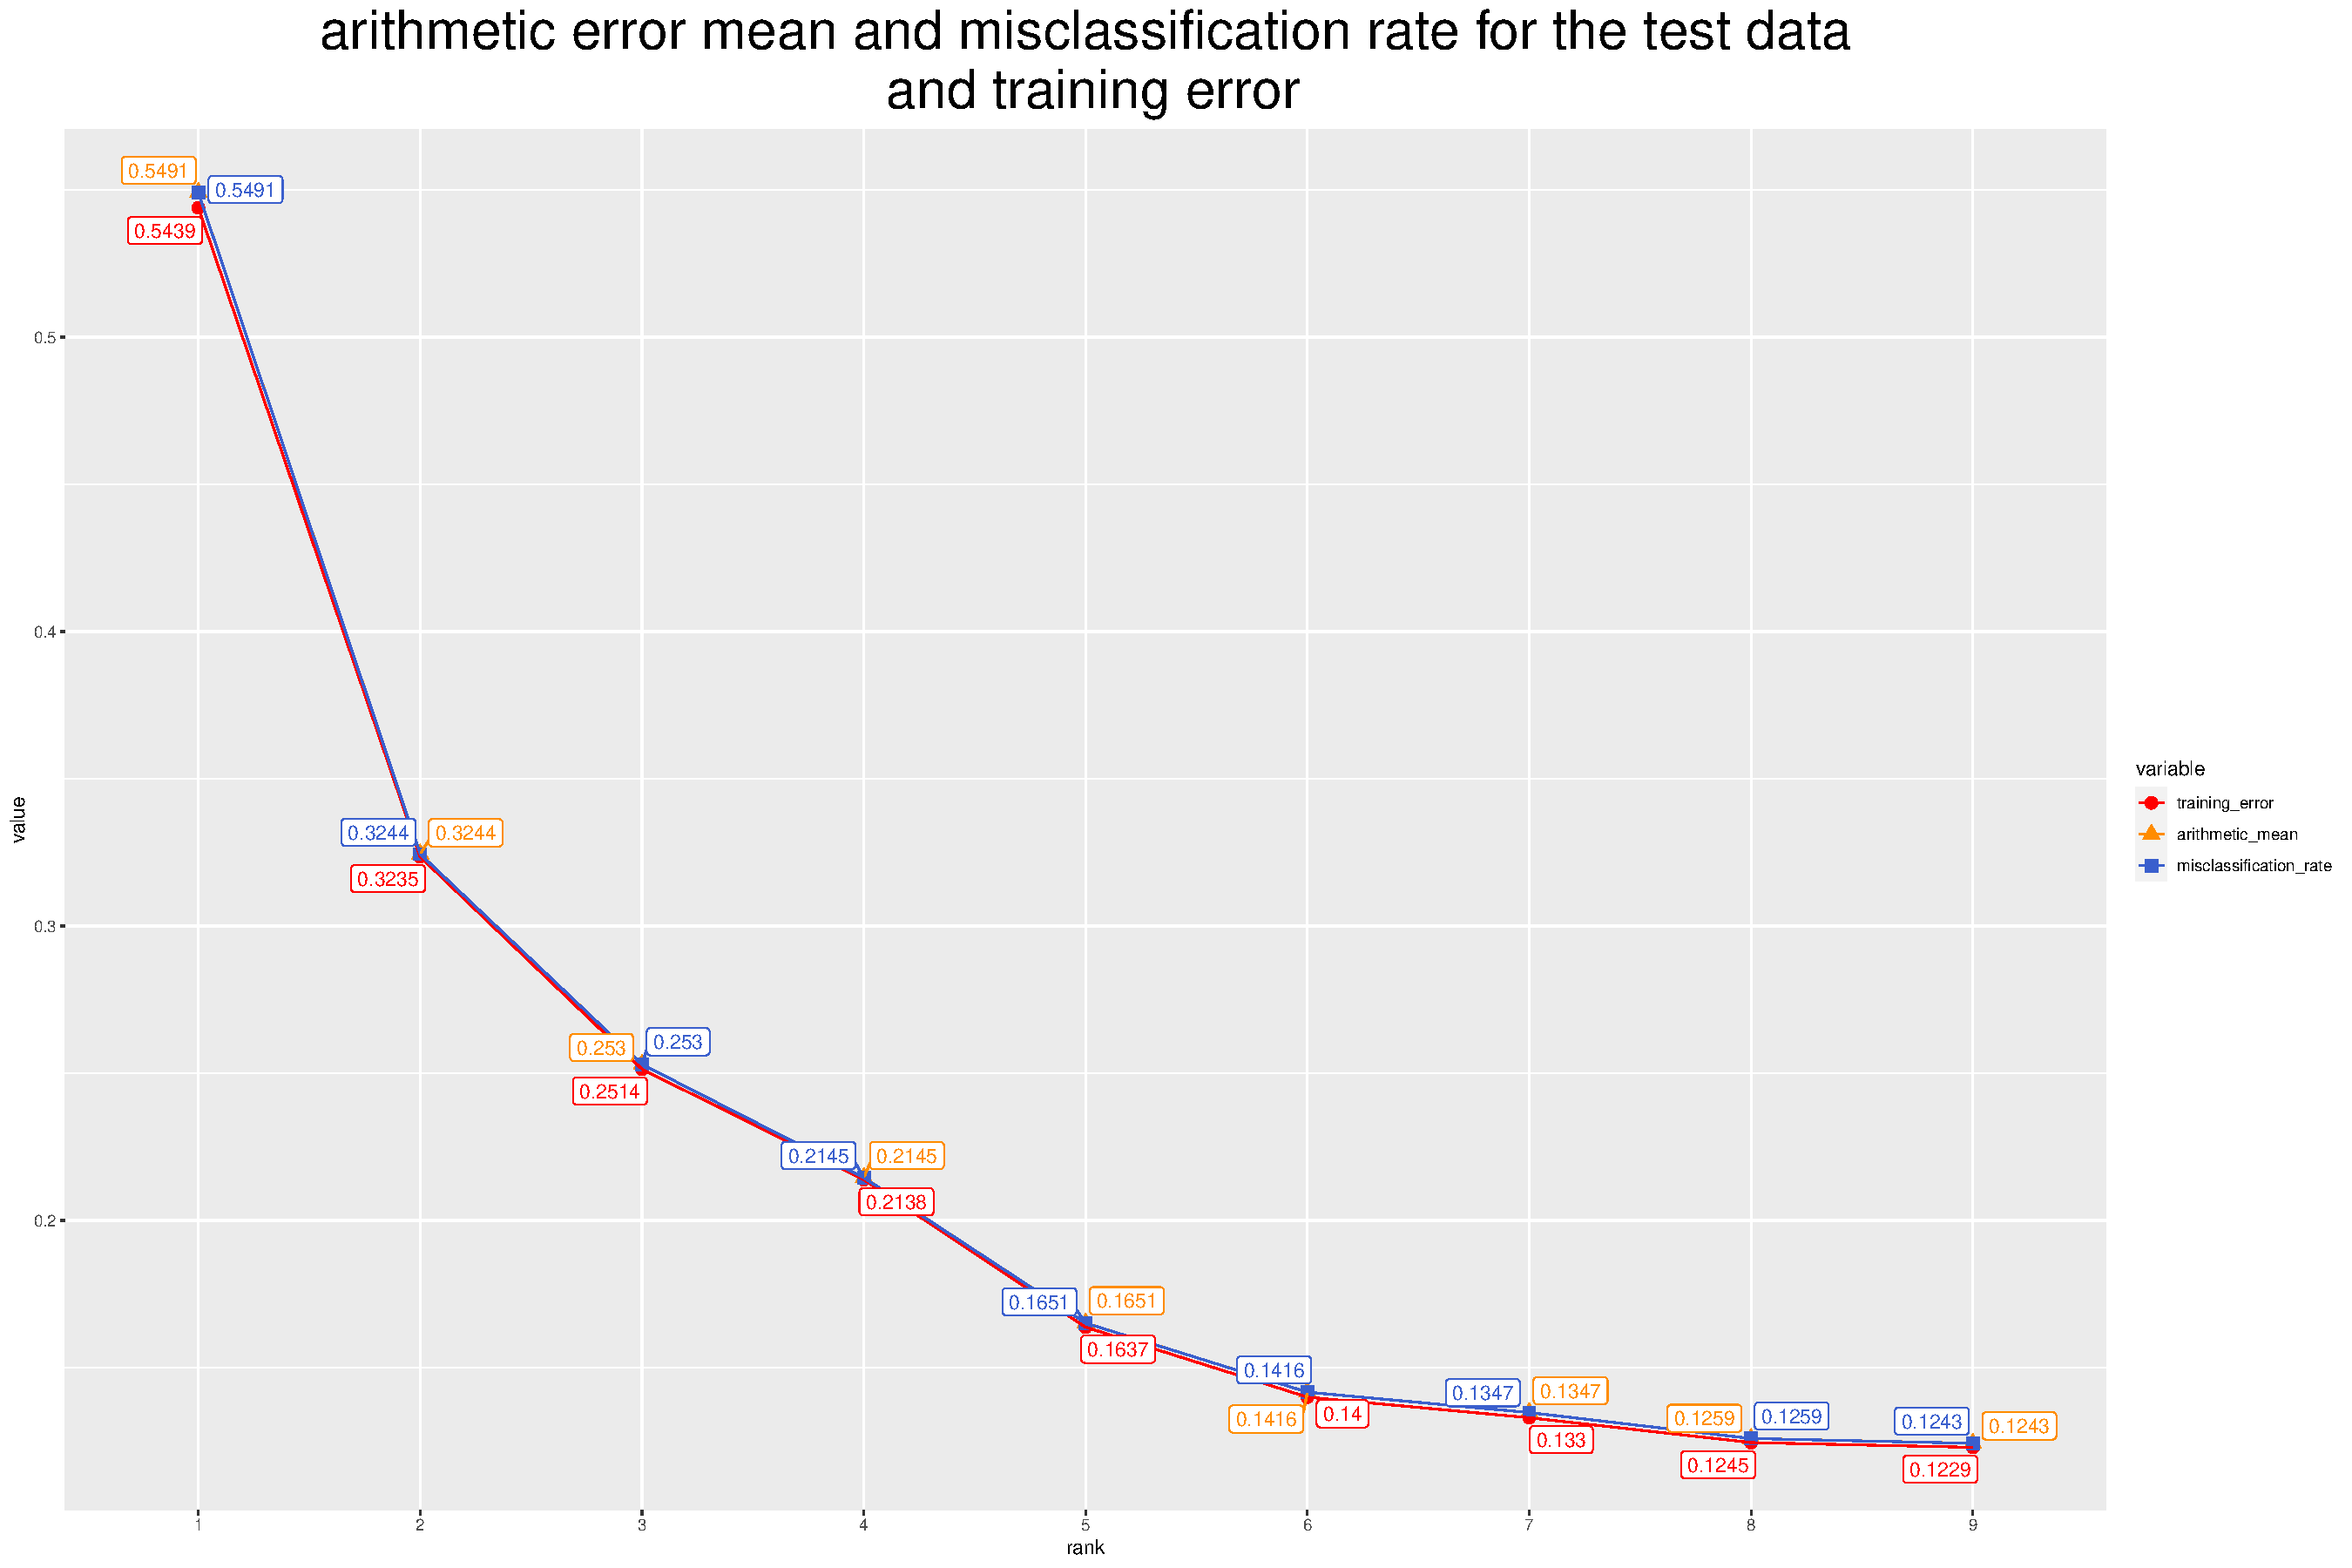
\includegraphics{ProblemSet2_files/figure-pdf/unnamed-chunk-77-1.pdf}

We can see that the cross validation error keeps improving as the number
of dimensions grows, which suggests that all linear discriminant
directions matter for classification purposes - albeit to different
extents. We could make a case for keeping only 6 dimensions if we
focused on dimensionality reduction, following a sort of ``elbow rule''.
Overall, the most balanced decision is to keep all 9 dimensions.

\hypertarget{optional-find-a-classification-rule-that-improves-on-the-cv-error-rate-estimates-found-before.-feel-free-to-use-any-classification-method-even-one-not-covered-in-class.}{%
\subsubsection{\texorpdfstring{5. \((optional)\) Find a classification
rule that improves on the CV error rate estimates found before. Feel
free to use any classification method, even one not covered in
class.}{5. (optional) Find a classification rule that improves on the CV error rate estimates found before. Feel free to use any classification method, even one not covered in class.}}\label{optional-find-a-classification-rule-that-improves-on-the-cv-error-rate-estimates-found-before.-feel-free-to-use-any-classification-method-even-one-not-covered-in-class.}}

Since the assumption of equal covariance matrix across classes seems
stretched, our first thought is simply to try Quadratic Discriminant
Analysis, which doesn't require it. Note that we wouldn't expect a huge
improvement, since it would still rely on the assumption of Gaussian
conditional densities.

QDA is, however, impossible to implement in this case. Indeed, QDA
requires invertibility of all the sample covariance matrices in its
procedure, not only of the pooled one, and digit \emph{4} doesn't have a
full rank covariance matrix (as previously discussed).

\begin{Shaded}
\begin{Highlighting}[]
\NormalTok{qda.fit}\OtherTok{=}\FunctionTok{qda}\NormalTok{(digit}\SpecialCharTok{\textasciitilde{}}\NormalTok{.,}\AttributeTok{data=}\NormalTok{pendigits, }\AttributeTok{CV=}\ConstantTok{TRUE}\NormalTok{)}
\end{Highlighting}
\end{Shaded}

\begin{verbatim}
Error in qda.default(x, grouping, ...): carenza di rango nel gruppo 4
\end{verbatim}

Before switching to another framework, we could try and implement a
similar procedure that ignores the problem of the singularity of the
covariance matrix of digit \emph{4}: Regularized Discriminant Analysis.
This technique is in between LDA and QDA, in the sense that it relies on
class covariance matrix estimates that are given by a linear combination
of the pooled covariance matrix and of the sample covariance matrix of
the considered class. The coefficients of the combinations are estimated
as to minimize the error rates by default. Quite unexpectedly, the
improvements achieved via a 44-fold Cross Validation RDA on the LDA
error rates are astounding - where we used again a 44-fold cross
validation technique to make error estimates more comparable with the
previous ones.

\begin{Shaded}
\begin{Highlighting}[]
\NormalTok{rda.fit}\OtherTok{=}\FunctionTok{rda}\NormalTok{(digit}\SpecialCharTok{\textasciitilde{}}\NormalTok{.,}\AttributeTok{data=}\NormalTok{pendigits, }\AttributeTok{crossval=}\ConstantTok{TRUE}\NormalTok{, }\AttributeTok{fold=}\DecValTok{44}\NormalTok{)}
\NormalTok{rda.fit}\SpecialCharTok{$}\NormalTok{error.rate}
\end{Highlighting}
\end{Shaded}

\begin{verbatim}
      APER   crossval 
0.01455604 0.01545961 
\end{verbatim}

Here ``APER'' (apparent error rate) corresponds to what we called
``total misclassification rates'' above, and ``crossval'' is the cross
validation error. The errors are almost reduced by a \(\frac{1}{10}\)
factor compared to LDA.

Since relying less on the assumptions of LDA provides us an improved
outcome, the next technique we implement is Multinomial Logistic
Regression (a generalisation of the standard Binomial Logistic
Regression for categorical variables with more than 2 possible
outcomes). Indeed, the strategy is almost identical to the one of LDA
(maximization of the discriminant functions), but it relies on the
weaker assumptions of logistic regression (the log-odds of each class is
assumed to be a linear combination of the explanatory variables). We
repeat k-fold CV on this model using the same criterion above.

\begin{Shaded}
\begin{Highlighting}[]
\NormalTok{mlog.err}\OtherTok{=}\DecValTok{0}
\NormalTok{mlog.mis}\OtherTok{=}\DecValTok{0}
\ControlFlowTok{for}\NormalTok{(i }\ControlFlowTok{in} \DecValTok{1}\SpecialCharTok{:}\NormalTok{k\_f)\{}
  \FunctionTok{set.seed}\NormalTok{(i) }\CommentTok{\#random initial parameters, different for each cycle}
\NormalTok{  train }\OtherTok{=} \SpecialCharTok{!}\NormalTok{(groupCV}\SpecialCharTok{==}\NormalTok{i)}
\NormalTok{  train.data}\OtherTok{=}\NormalTok{pendigits[train,]}
\NormalTok{  test.data}\OtherTok{=}\NormalTok{pendigits[}\SpecialCharTok{!}\NormalTok{train,]}
\NormalTok{  mlog.model }\OtherTok{=}\NormalTok{ nnet}\SpecialCharTok{::}\FunctionTok{multinom}\NormalTok{(digit }\SpecialCharTok{\textasciitilde{}}\NormalTok{., }\AttributeTok{data =}\NormalTok{ train.data)}
\NormalTok{  pred.classes }\OtherTok{=}\NormalTok{ mlog.model }\SpecialCharTok{\%\textgreater{}\%} \FunctionTok{predict}\NormalTok{(test.data)}
\NormalTok{  mlog.err}\OtherTok{=}\NormalTok{mlog.err}\SpecialCharTok{+}\DecValTok{1}\SpecialCharTok{{-}}\FunctionTok{mean}\NormalTok{(pred.classes }\SpecialCharTok{==}\NormalTok{ test.data}\SpecialCharTok{$}\NormalTok{digit)}
\NormalTok{  mlog.mis}\OtherTok{=}\NormalTok{mlog.mis}\SpecialCharTok{+}\FunctionTok{sum}\NormalTok{(}\SpecialCharTok{!}\NormalTok{train)}\SpecialCharTok{{-}}\FunctionTok{sum}\NormalTok{(pred.classes }\SpecialCharTok{==}\NormalTok{ test.data}\SpecialCharTok{$}\NormalTok{digit) }
  \CommentTok{\#number of misclassifications as the total number of test data {-} }
  \CommentTok{\#the correctly predicted class}
\NormalTok{\}}
\NormalTok{mlog.err}\OtherTok{=}\NormalTok{mlog.err}\SpecialCharTok{/}\NormalTok{k\_f }\CommentTok{\#error by means of the errors}

\NormalTok{mlog.mis}\OtherTok{=}\NormalTok{mlog.mis}\SpecialCharTok{/}\NormalTok{n}
\end{Highlighting}
\end{Shaded}

\begin{verbatim}
  Arithmetic.average.of.errors Misclassification.rate
1                   0.07996619             0.07996725
\end{verbatim}

The results are good, but not as good as those of RDA. Furthermore, the
function used to implement this Multinomial Logistic Regression relies
on a random choice of initial parameters and the outcome is sensitive to
the choice of these initial values.

We also attempt to use a random forest, a popular classification method
that performs very well on many classification tasks. Usually the great
advantage of random forests is the interpretability of the model, which
in this case is quite secondary, but it's still worth checking if the
errors improve. We tried tuning the parameters for the random forest but
we did not find significant improvements, so we kept the default ones
(\texttt{ntree}=500, \texttt{mtry}=4).

\begin{Shaded}
\begin{Highlighting}[]
\NormalTok{rfor.err}\OtherTok{=}\DecValTok{0}
\NormalTok{rfor.mis}\OtherTok{=}\DecValTok{0}
\ControlFlowTok{for}\NormalTok{(i }\ControlFlowTok{in} \DecValTok{1}\SpecialCharTok{:}\NormalTok{k\_f)\{}
  \FunctionTok{set.seed}\NormalTok{(i)}
\NormalTok{  train }\OtherTok{=} \SpecialCharTok{!}\NormalTok{(groupCV}\SpecialCharTok{==}\NormalTok{i)}
\NormalTok{  train.data}\OtherTok{=}\NormalTok{pendigits[train,]}
\NormalTok{  train.data}\SpecialCharTok{$}\NormalTok{digit}\OtherTok{=}\FunctionTok{as.factor}\NormalTok{(train.data}\SpecialCharTok{$}\NormalTok{digit)}
\NormalTok{  test.data}\OtherTok{=}\NormalTok{pendigits[}\SpecialCharTok{!}\NormalTok{train,]}
\NormalTok{  test.data}\SpecialCharTok{$}\NormalTok{digit}\OtherTok{=}\FunctionTok{as.factor}\NormalTok{(test.data}\SpecialCharTok{$}\NormalTok{digit)}
\NormalTok{  rfor.model }\OtherTok{=} \FunctionTok{randomForest}\NormalTok{(digit }\SpecialCharTok{\textasciitilde{}}\NormalTok{., }\AttributeTok{data =}\NormalTok{ train.data)}
\NormalTok{  pred.classes }\OtherTok{=} \FunctionTok{predict}\NormalTok{(rfor.model, test.data)}
\NormalTok{  rfor.err}\OtherTok{=}\NormalTok{rfor.err}\SpecialCharTok{+}\FunctionTok{mean}\NormalTok{(pred.classes }\SpecialCharTok{!=}\NormalTok{ test.data}\SpecialCharTok{$}\NormalTok{digit)}
\NormalTok{  rfor.mis}\OtherTok{=}\NormalTok{rfor.mis}\SpecialCharTok{+}\FunctionTok{sum}\NormalTok{(pred.classes }\SpecialCharTok{!=}\NormalTok{ test.data}\SpecialCharTok{$}\NormalTok{digit) }
\NormalTok{\}}
\NormalTok{rfor.err}\OtherTok{=}\NormalTok{rfor.err}\SpecialCharTok{/}\NormalTok{k\_f }\CommentTok{\#error as means of the errors}
\NormalTok{rfor.mis}\OtherTok{=}\NormalTok{rfor.mis}\SpecialCharTok{/}\NormalTok{n}

\FunctionTok{data.frame}\NormalTok{(}\StringTok{"Arithmetic average of errors"} \OtherTok{=}\NormalTok{ rfor.err,}
           \StringTok{"Misclassification rate"} \OtherTok{=}\NormalTok{ rfor.mis) }
\end{Highlighting}
\end{Shaded}

\begin{verbatim}
  Arithmetic.average.of.errors Misclassification.rate
1                  0.007736289            0.007732897
\end{verbatim}

Random forests perform better than all previously considered methods.

At last, we mention that we also tried to use the more ``naive'' method
of the k-Nearest Neighbors, which yielded surprisingly good results for
small values of k. We show the error rates for k from \(1\) to \(10\),
but up to \(100\) they only increased along with k, so the optimal
choice appear to be either \(1\) or \(3\). This behavior was not
completely predictable: the error rate is usually an increasing function
of k when computed on training data, yet it still happens the same
despite testing the model on test data - not used for training - via
cross-validation.

\begin{Shaded}
\begin{Highlighting}[]
\FunctionTok{set.seed}\NormalTok{(}\DecValTok{1}\NormalTok{)}
\NormalTok{knn.err}\OtherTok{=}\FunctionTok{numeric}\NormalTok{(}\DecValTok{10}\NormalTok{)}
\NormalTok{knn.mis}\OtherTok{=}\FunctionTok{numeric}\NormalTok{(}\DecValTok{10}\NormalTok{)}
\ControlFlowTok{for}\NormalTok{(aux }\ControlFlowTok{in} \DecValTok{1}\SpecialCharTok{:}\DecValTok{10}\NormalTok{)\{}
\NormalTok{  knn.err\_tmp}\OtherTok{=}\DecValTok{0}
\NormalTok{  knn.mis\_tmp}\OtherTok{=}\DecValTok{0}
  \ControlFlowTok{for}\NormalTok{(i }\ControlFlowTok{in} \DecValTok{1}\SpecialCharTok{:}\NormalTok{k\_f)\{}
\NormalTok{    train }\OtherTok{=} \SpecialCharTok{!}\NormalTok{(groupCV}\SpecialCharTok{==}\NormalTok{i)}
\NormalTok{    train.data}\OtherTok{=}\NormalTok{pendigits[train,]}
\NormalTok{    train.data}\SpecialCharTok{$}\NormalTok{digit}\OtherTok{=}\FunctionTok{as.factor}\NormalTok{(train.data}\SpecialCharTok{$}\NormalTok{digit)}
\NormalTok{    test.data}\OtherTok{=}\NormalTok{pendigits[}\SpecialCharTok{!}\NormalTok{train,]}
\NormalTok{    test.data}\SpecialCharTok{$}\NormalTok{digit}\OtherTok{=}\FunctionTok{as.factor}\NormalTok{(test.data}\SpecialCharTok{$}\NormalTok{digit)}
\NormalTok{    knn.pred }\OtherTok{=}\NormalTok{ class}\SpecialCharTok{::}\FunctionTok{knn}\NormalTok{(}\AttributeTok{train=}\NormalTok{train.data[,}\DecValTok{1}\SpecialCharTok{:}\DecValTok{16}\NormalTok{], }\AttributeTok{cl=}\NormalTok{train.data[,}\DecValTok{17}\NormalTok{],}
                          \AttributeTok{test=}\NormalTok{test.data[,}\DecValTok{1}\SpecialCharTok{:}\DecValTok{16}\NormalTok{], }\AttributeTok{k=}\NormalTok{aux)}
\NormalTok{    knn.err\_tmp}\OtherTok{=}\NormalTok{knn.err\_tmp}\SpecialCharTok{+}\FunctionTok{mean}\NormalTok{(knn.pred }\SpecialCharTok{!=}\NormalTok{ test.data}\SpecialCharTok{$}\NormalTok{digit)}
\NormalTok{    knn.mis\_tmp}\OtherTok{=}\NormalTok{knn.mis\_tmp}\SpecialCharTok{+}\FunctionTok{sum}\NormalTok{(knn.pred }\SpecialCharTok{!=}\NormalTok{ test.data}\SpecialCharTok{$}\NormalTok{digit) }
\NormalTok{  \}}
\NormalTok{  knn.err[aux]}\OtherTok{=}\NormalTok{knn.err\_tmp}\SpecialCharTok{/}\NormalTok{k\_f}
\NormalTok{  knn.mis[aux]}\OtherTok{=}\NormalTok{knn.mis\_tmp}\SpecialCharTok{/}\NormalTok{n}
\NormalTok{\}}
\end{Highlighting}
\end{Shaded}

\begin{verbatim}
    k Arithmetic.average.of.errors Misclassification.rate
1   1                  0.006275733            0.006277293
2   2                  0.006548460            0.006550218
3   3                  0.006369647            0.006368268
4   4                  0.006736289            0.006732169
5   5                  0.007378663            0.007368996
6   6                  0.007736289            0.007732897
7   7                  0.008012021            0.008005822
8   8                  0.008557476            0.008551674
9   9                  0.009466566            0.009461426
10 10                  0.010469572            0.010462154
\end{verbatim}

In terms of raw error rates, k-NN should be our best choice. However,
due to its instability, we should probably opt for Random Forests
regardless.



\end{document}
